%%%%%%%%%%%%%%%%%%%%%%%%%%%%%%%%%%%%%%%%%%%%%%%%%%%%%%%%%%%%%%%%%%%%%%%%%%%%%%%%
%%%%%%%%%%%%%%%%%%%%%%%%%%%%%%%%%%%%%%%%%%%%%%%%%%%%%%%%%%%%%%%%%%%%%%%%%%%%%%%%
%%                                                                            %%
%% thesistemplate_short.tex version 4.21 (2026/02/19)                         %%
%%                                                                            %%
%%%%%%%%%%%%%%%%%%%%%%%%%%%%%%%%%%%%%%%%%%%%%%%%%%%%%%%%%%%%%%%%%%%%%%%%%%%%%%%%
\documentclass[english, 12pt, a4paper, elec, utf8, a-2b, online]{aaltothesis}
%\documentclass[english, 12pt, a4paper, elec, utf8, a-2b, print]{aaltothesis}
%\documentclass[english, 12pt, a4paper, elec, utf8, a-2b, print, twoside]{aaltothesis}

%\usepackage[options]{amsmath}
%\usepackage{amsthm}

%% DO NOT MOVE OR REMOVE \setupthesisfonts
\setupthesisfonts

\usepackage{graphicx}
\usepackage{amsmath}
\usepackage{longtable}
\usepackage{array}
\newcolumntype{L}[1]{>{\raggedright\arraybackslash}p{#1}}
\usepackage{placeins}
\usepackage[type={CC}, modifier={by-nc-sa}, version={4.0}]{doclicense}

\usepackage[
backend=biber,
style=numeric-comp,
sorting=nyt,
firstinits=true,
urldate=long
]{biblatex}
\addbibresource{thesisreferences.bib}

\usepackage{xcolor}

%% -----------------------------------------------------------------------
%% ONLY THE LINES BELOW ARE CHANGED FROM THE ORIGINAL TEMPLATE
%% -----------------------------------------------------------------------

\degreeprogram{ICT Innovation}

\major{Autonomous Systems and Intelligent Robots}

\univdegree{MSc}
%\univdegree{BSc}
%\univdegree{Lic}

\thesisauthor{Xinle Zhang}

\thesistitle{Dynamic Environment State Estimation for Multi-Agent Systems under Partial Macroscopic Observations}

\thesissubtitle{}

\place{Espoo}

\date{November 2026}

\supervisor{Prof.\ Tomasz Kucner}

\advisor{Maryam Kazemi Eskeri}

\advisor{Joona Manninen}

%\collaborativepartner{Company or institute name (if relevant)}

\uselogo{'}

\copyrighttext{\noexpand\textcopyright\ \number\year. This work is
	licensed under a Creative Commons "Attribution-NonCommercial-ShareAlike 4.0
	International" (BY-NC-SA 4.0) license.}{\noindent\textcopyright\ \number
	\year \ \doclicenseThis}

\keywords{state estimation\spc uncertainty quantification\spc crowd state reconstruction\spc multi-robot systems\spc data assimilation\spc partial observations}

% PDF/A metadata must be a single paragraph: blank lines generate \par.
\thesisabstract{%
Understanding the overall state of a pedestrian crowd is challenging when
observations cover only parts of the environment. Robots in crowded public spaces have limited sensor coverage,
making it difficult to estimate pedestrians outside their individual perception
ranges. Multiple robots can share observations from different parts of the
environment, as local, aggregated measurements such as pedestrian density and
mean velocity. However, these measurements are incomplete, and reconstructing
the global crowd state from them requires estimating both the full state of the
crowd and the uncertainty associated with that estimate. Methods from data
assimilation and sparse field reconstruction address such problems in other
domains, but to the best of our knowledge, their performance on crowd state
estimation has not been reported.
This thesis addresses how accurately such methods reconstruct a crowd's
macroscopic state from the partial observations of mobile robots, the quality
of the uncertainty, and their computational cost. It
compares a localised Ensemble Kalman Filter (EnKF), DINCAE, Senseiver and
4DVarNet using the ATC dataset, 92 days of real pedestrian data, observed by
three robots. Two extensions
are proposed: since Senseiver uses only the current
frame, although most currently unobserved cells were observed seconds earlier,
Senseiver-G aligns its latent representation with the grid and adds a causal
window of past observations; since 4DVarNet provides no uncertainty, an
augmented 4DVarNet refines the state and its log-variance jointly within its
trained solver.
Senseiver-G is the most accurate of the six methods on every state channel. On
the 15 test days, its RMSE on the walkable cells, pooled over the four state
channels, is 12.7 percent below that of the original Senseiver. Among the probabilistic methods, DINCAE gives
the best predictive distribution, with the lowest
continuous ranked probability score on every test day, helped by its accurate point estimate. The augmented
4DVarNet provides an uncertainty for a quarter more computation than the plain
4DVarNet but, in the reported run, is less accurate. The compute time per
frame differs by more than two orders of magnitude between the methods and is
far below the one-second observation interval, but it is not the end-to-end
latency: it excludes input preparation and, for DINCAE and 4DVarNet, the wait
for later observations.
}

%\setboolean{writexmpdatafile}{false}

%% -----------------------------------------------------------------------
%% END OF CHANGES
%% -----------------------------------------------------------------------


\begin{document}

\makecoverpage

\makecopyrightpage

\clearpage

%% English abstract
\begin{abstractpage}[english]
Understanding the overall state of a pedestrian crowd is challenging when
observations cover only parts of the environment. Robots in crowded public spaces have limited sensor coverage,
making it difficult to estimate pedestrians outside their individual perception
ranges. Multiple robots can share observations from different parts of the
environment, as local, aggregated measurements such as pedestrian density and
mean velocity. However, these measurements are incomplete, and reconstructing
the global crowd state from them requires estimating both the full state of the
crowd and the uncertainty associated with that estimate. Methods from data
assimilation and sparse field reconstruction address such problems in other
domains, but to the best of our knowledge, their performance on crowd state
estimation has not been reported.

This thesis addresses how accurately such methods reconstruct a crowd's
macroscopic state from the partial observations of mobile robots, the quality
of the uncertainty, and their computational cost. It
compares a localised Ensemble Kalman Filter (EnKF), DINCAE, Senseiver and
4DVarNet using the ATC dataset, 92 days of real pedestrian data, observed by
three robots. Two extensions
are proposed: since Senseiver uses only the current
frame, although most currently unobserved cells were observed seconds earlier,
Senseiver-G aligns its latent representation with the grid and adds a causal
window of past observations; since 4DVarNet provides no uncertainty, an
augmented 4DVarNet refines the state and its log-variance jointly within its
trained solver.

Senseiver-G is the most accurate of the six methods on every state channel. On
the 15 test days, its RMSE on the walkable cells, pooled over the four state
channels, is 12.7\% below that of the original Senseiver. Among the probabilistic methods, DINCAE gives
the best predictive distribution, with the lowest
continuous ranked probability score on every test day, helped by its accurate point estimate. The augmented
4DVarNet provides an uncertainty for a quarter more computation than the plain
4DVarNet but, in the reported run, is less accurate. The compute time per
frame differs by more than two orders of magnitude between the methods and is
far below the one-second observation interval, but it is not the end-to-end
latency: it excludes input preparation and, for DINCAE and 4DVarNet, the wait
for later observations.

\end{abstractpage}

%\begin{abstractpage}[english]
%	\abstracttext{}
%\end{abstractpage}




\dothesispagenumbering{}

%% Preface
\mysection{Preface}
I want to thank my supervisor, Professor Tomasz Kucner, and my advisors, Maryam Kazemi Eskeri of Aalto University and Joona Manninen of Propia Services Oy, for their guidance throughout this work.

The computations in this thesis were performed with the computing resources provided by the Aalto Science-IT project.

AI tools (Claude by Anthropic and ChatGPT by OpenAI) were used in this thesis to assist in searching for literature, in writing and revising the text, and in writing and debugging code. I have reviewed all the content and take full responsibility for it.

\vspace{5cm}
Otaniemi, 3 November 2026\\

\vspace{5mm}
{\hfill Xinle Zhang \hspace{1cm}}

\newpage

\thesistableofcontents

%% Symbols and abbreviations
\mysection{Symbols and abbreviations}

\subsection*{Symbols}

Only the symbols used throughout the thesis are listed; symbols that belong to
one method are defined where they are introduced.

\begin{longtable}{p{0.2\textwidth}L{0.72\textwidth}}
$H, W$                    & number of grid rows and columns ($36 \times 12$ cells of 1\,m) \\
$t$                       & time (frame index, one frame per second) \\
$t'$                      & time of an observation used to reconstruct frame $t$ \\
$x_t$                     & crowd state at time $t$, $x_t \in \mathbb{R}^{4 \times H \times W}$ \\
$\rho$                    & pedestrian density [people/m$^2$] \\
$v_x, v_y$                & mean walking velocity along and across the corridor [m/s] \\
$\nu$                     & velocity variance [m$^2$/s$^2$] \\
$\mathcal{W}$             & set of walkable cells \\
$\Omega_t$                & observation mask at time $t$ (1 = observed) \\
$\mathcal{B}_t$           & blind cells: walkable cells not observed at time $t$ \\
$y_t$                     & observation at time $t$ \\
$\varepsilon_t$           & observation noise \\
$\sigma_{\mathrm{obs}}$   & per-channel standard deviation of the observation noise \\
$\hat{x}_t$               & reconstructed state (point estimate) \\
$\hat{\sigma}_t$          & predicted standard deviation (uncertainty) of $\hat{x}_t$ \\
\end{longtable}

\subsection*{Operators}

\begin{longtable}{p{0.2\textwidth}L{0.72\textwidth}}
$\odot$                          & element-wise product \\
$\ast$                           & convolution \\
$\nabla_x J$                     & gradient of $J$ with respect to $x$ \\
$\|\cdot\|_{W_{\mathrm{obs}}}, \|\cdot\|_{W_{\mathrm{reg}}}$ & norm weighted by the per-channel coefficients $W_{\mathrm{obs}}$ or $W_{\mathrm{reg}}$ \\
$\|\cdot\|_{\mathrm{rms}}$       & root-mean-square over all elements \\
$|\mathcal{A}|$                  & number of elements of a set $\mathcal{A}$ \\
$[\,a,\ b\,]$                    & concatenation \\
$\mathcal{N}(\mu, \sigma^2)$     & normal distribution with mean $\mu$ and variance $\sigma^2$ \\
$\mathrm{diag}(\cdot)$           & diagonal matrix with the given diagonal \\
\end{longtable}

\subsection*{Abbreviations}

\begin{longtable}{p{0.2\textwidth}L{0.72\textwidth}}
A$^*$      & A-star shortest-path search algorithm \\
AR(1)      & autoregressive process of order one \\
ATC        & Asia and Pacific Trade Center (shopping centre in Osaka, Japan) \\
CNN        & convolutional neural network \\
ConvLSTM   & convolutional long short-term memory \\
CPU        & central processing unit \\
CRPS       & continuous ranked probability score \\
DINCAE     & Data-Interpolating Convolutional Auto-Encoder \\
DIVAnd     & Data-Interpolating Variational Analysis in $n$ dimensions \\
EnKF       & Ensemble Kalman Filter \\
GELU       & Gaussian error linear unit \\
GENN       & Gibbs-energy neural network \\
GPU        & graphics processing unit \\
GRU        & gated recurrent unit \\
LN         & layer normalisation \\
LR         & learning rate \\
LReLU      & leaky rectified linear unit \\
LSTM       & long short-term memory \\
MC-Dropout & Monte Carlo dropout \\
MHA        & multi-head attention \\
MLP        & multi-layer perceptron \\
MSE        & mean squared error \\
NLL        & negative log-likelihood \\
PE         & position encoding \\
ReLU       & rectified linear unit \\
RMS        & root-mean-square \\
RMSE       & root-mean-square error \\
RQ         & research question \\
SHRED      & shallow recurrent decoder \\
SPDE       & stochastic partial differential equation \\
SSH        & sea surface height \\
\end{longtable}
% longtable steps the table counter even without a caption
\setcounter{table}{0}


\cleardoublepage

\section{Introduction}
\label{sec:intro}

%% ------------------------------------------------------------------
%% 1. Motivation: broad context
%% ------------------------------------------------------------------

Environments shared by humans and autonomous agents, such as pedestrian
plazas, shopping centres and transport hubs, are often crowded, and their state
changes continuously. An estimate of how the crowd as a whole is distributed
and moving is useful to any agent that operates there, but no single agent can
observe it: each perceives only the part of the environment within its own
sensing range. In principle, the global state could be assembled if the
individual positions and velocities of all pedestrians, and the observations of
every agent, were available. In practice, however, this level of detail is
rarely available: sensing range is limited, and privacy or hardware
limitations often mean that only \emph{partial and aggregated}
information can be observed, such as local pedestrian density,
average flow velocity, or coarse occupancy patterns.

The estimation task is to reconstruct the macroscopic crowd field, including
its unobserved parts, from local, noisy measurements. The macroscopic
description is chosen because the environments of interest are dense:
estimating and tracking every individual is costly there and often not
possible, whereas aggregated quantities such as density and mean flow describe
the crowd with a number of values that does not grow with the number of people
and that identifies no individual. The reconstruction is an ill-posed inverse
problem: different fields in unobserved regions can produce the same local
observations. Nonlinear dynamics that are not known in advance, several moving
agents with different partial views, and the dimension of the state --
1\,728 values per second in this thesis, of which the robots observe only a
part -- make reconstruction harder. An estimate of the uncertainty of the
reconstruction is useful as well, since any later use of the reconstructed
field can then take its errors into account.

%% ------------------------------------------------------------------
%% 2. Precise problem definition and identification of the gap
%% ------------------------------------------------------------------

This thesis focuses on the problem of \emph{environment state estimation for
multi-agent systems under partial macroscopic observations}: given a
set of agents that each observe only a spatially limited, aggregated
view of a shared dynamic environment (e.g., local density and flow
statistics rather than individual positions), the goal is to combine
these partial observations into an estimate of the global state of
the environment. Because an estimate is more useful when its reliability is
known, the thesis
additionally examines the uncertainty that some of the methods provide
alongside the state, and the computational cost of producing both.

Existing approaches to the underlying reconstruction problem fall
into two broad categories. \emph{Ensemble-based Bayesian filtering},
exemplified by the Ensemble Kalman Filter (EnKF), represents the
state distribution with a finite ensemble of samples propagated
through a forward model and corrected using incoming observations
\cite{roth2017enkf}; it does not require the forward model to
be linearised, and represents uncertainty naturally through the spread
of its ensemble, but its accuracy and computational cost depend on
the ensemble size and the forward model used to propagate it.
\emph{Learned, data-driven reconstruction methods} instead train a
model end-to-end on historical data, and at inference time apply the trained
model with its weights fixed: direct reconstruction networks in one forward
evaluation, learned variational methods in a fixed sequence of gradient
calculations with respect to the state and learned updates. This category includes both direct sparse field
reconstruction networks, such as the Data-Interpolating Convolutional
Auto-Encoder (DINCAE) \cite{barth2022dincae2} and
Senseiver \cite{santos2023senseiver}, and learned variational assimilation
schemes, such as 4DVarNet \cite{fablet2020fourdvarnet}, which retain the
structure of a variational data-assimilation cost function but
parametrise its components with neural networks trained from data.

The learned methods were developed and validated in other domains:
4DVarNet, like the variational assimilation methods it builds on,
mainly on geophysical and oceanographic fields, and DINCAE and
Senseiver on satellite and fluid-dynamics data. The reviewed literature does
not report their evaluation on the problem addressed in this
thesis (Section~\ref{sec:methods}): a crowd's macroscopic state
reconstructed from the partial observations of a team of mobile robots.
Applying them to this problem is therefore a question of domain adaptation. In
this thesis, domain adaptation refers to adapting the methods -- their inputs,
architectures and training -- to the crowd domain and training them on crowd
data; no model trained in another domain is transferred. Whether the methods
can be adapted in this way, and how they then compare in the accuracy of the
reconstructed state and in the quality of the uncertainty that some of them
provide, is not known. The methods also differ in whether they provide an
uncertainty at all: the EnKF represents it through the spread of its
ensemble and DINCAE learns an error variance, whereas Senseiver and
4DVarNet produce only a point estimate. General-purpose ways of adding
an uncertainty to a learned model, such as Deep Ensembles
\cite{lakshminarayanan2017deepensembles} and Monte Carlo dropout (MC-Dropout)
\cite{gal2016mcdropout}, do so by training several networks or by
running several stochastic forward passes.

This thesis compares, on a common problem using a real pedestrian
dataset, a localised EnKF with three learned methods -- DINCAE,
Senseiver and 4DVarNet -- and proposes two extensions. The first
integrates an uncertainty estimate into a learned variational
assimilation model (4DVarNet), such that a single model produces both a
state estimate and its uncertainty in one complete solver invocation; for its
uncertainty, it is compared with the EnKF, which represents uncertainty
through its ensemble, and with DINCAE, which learns its error variance
directly, and for its accuracy with the plain 4DVarNet. The second
extends the reference Senseiver architecture, which reconstructs every frame
from that frame's observations alone, so that it can use the
observations collected over the preceding seconds, during which the moving
robots have seen most of the currently unobserved cells; for
its accuracy, it is compared with the reference Senseiver.

%% ------------------------------------------------------------------
%% 3. Why this matters
%% ------------------------------------------------------------------

Any downstream use of the estimate, for example in navigation or in the
coordination of several agents, benefits from both an accurate state estimate
and a predictive distribution that represents its errors reliably. This motivates evaluating
probabilistic predictions with a proper scoring rule and checking the overall
scale of their predicted spread and the coverage of their prediction intervals. An estimator used online must also be causal:
it can use only observations that have already arrived, which makes recent
past observations particularly valuable.

%% ------------------------------------------------------------------
%% 4. Comparison criteria
%% ------------------------------------------------------------------

The evaluation in this thesis is conducted along three axes:

\begin{itemize}
    \item \textbf{Reconstruction accuracy}: the root-mean-square error
    (RMSE) against the ground-truth state on all walkable cells, and separately on the cells
    that no agent observes, for all methods under identical observations.
    \item \textbf{Uncertainty quality}: the continuous ranked
    probability score (CRPS), a proper scoring rule for the full predictive
    distribution, root-mean-square (RMS) predictive spread divided by point-estimate RMSE,
    which checks its overall size, and the coverage of its prediction
    intervals.
    \item \textbf{Computational cost}: inference time per
    reconstructed frame, compared directly across methods, since a state
    estimate and its uncertainty are useful online only if they are produced
    quickly enough.
\end{itemize}

%% ------------------------------------------------------------------
%% 5. Research questions
%% ------------------------------------------------------------------

Based on the problem definition above, this thesis addresses the
following research questions, one for each of the three axes above.
Each specifies the methods compared and the evaluation metric:

\begin{description}
    \item[RQ1 (accuracy)] Given partial, macroscopic observations of
    pedestrian density and flow, how accurately does each of the six
    methods -- a localised EnKF, DINCAE, Senseiver, 4DVarNet, and the
    two proposed extensions -- reconstruct the state over the
    walkable area, measured by the RMSE against the ground truth on all
    walkable cells and, separately, on the unobserved (blind) cells, under
    identical observations? In particular, how do the two proposed
    models compare with the methods they extend?
    \item[RQ2 (uncertainty)] For the three methods that predict an
    uncertainty -- the proposed uncertainty-aware 4DVarNet, the EnKF
    with its ensemble spread, and DINCAE with its learned error
    variance -- how good is the predicted uncertainty, measured by the
    CRPS of the predictive distribution, RMS spread divided by
    point-estimate RMSE, and the coverage of its 50\% and 90\% prediction
    intervals?
    \item[RQ3 (computational cost)] How much inference time does each
    of the six methods need per reconstructed frame, and what does the
    uncertainty output of the proposed 4DVarNet cost in time, relative to
    the plain 4DVarNet and to the EnKF?
\end{description}

%% ------------------------------------------------------------------
%% 6. Contribution statement
%% ------------------------------------------------------------------

The main contributions of this thesis are:

\begin{itemize}
    \item A comparison of existing state estimation methods -- a localised
    EnKF, DINCAE, Senseiver and 4DVarNet -- adapted from the domains they were
    developed in to crowd state estimation (domain adaptation), together with
    the two extensions below, on a common problem using a real pedestrian
    dataset observed by simulated robots, in terms of reconstruction accuracy,
    uncertainty quality and computational cost.
    \item An extension of the Senseiver sparse-reconstruction network,
    in which the latent array is aligned with the grid (one latent
    token per cell, read out directly) and the observations of the
    preceding seconds are encoded together with their time offsets,
    so that the model remains causal but can use recent observations
    of the currently unobserved cells.
    \item The design and implementation of an uncertainty estimation
    mechanism integrated into a learned variational data assimilation
    model (4DVarNet): the log-variance of the state is added to the
    variational state, both terms of the variational cost become Gaussian
    negative log-likelihoods in that variance, and the learned solver
    refines the variance together with the state, producing a state
    estimate and its marginal uncertainty within one invocation of the
    trained solver, comprising 20 learned updates.
\end{itemize}

%% ------------------------------------------------------------------
%% 7. Roadmap
%% ------------------------------------------------------------------

The remainder of this thesis is organised as follows.
Section~\ref{sec:background} introduces the concepts the methods rest
on: Bayesian state estimation, the Kalman filter and its ensemble
form, variational data assimilation, the neural network components
used, and the evaluation of probabilistic estimates.
Section~\ref{sec:related_work} reviews prior work grouped by
methodological approach: variational data assimilation, ensemble-based
sequential filtering, deep-learning-based sparse field reconstruction,
and uncertainty quantification for learned models.
Section~\ref{sec:methods} describes the research material (including
the dataset used to derive the partial macroscopic observations
and the simulated robots that observe it), the EnKF and the learned
methods, the two proposed models, and the protocol used to
evaluate them.
Section~\ref{sec:results} presents the results with respect to
RQ1--RQ3 and discusses them, and Section~\ref{sec:summary} gives the
conclusions and directions for future work.

\section{Background}
\label{sec:background}

This section introduces the concepts on which the methods of this thesis rest:
state estimation as Bayesian inference and its two classical solutions, the
Kalman filter with its ensemble form (Section~\ref{sec:bg_kalman}) and
variational data assimilation (Section~\ref{sec:bg_var}); the neural network
components used by the learned methods (Section~\ref{sec:bg_nn}); and the
evaluation of an estimate that comes with an uncertainty
(Section~\ref{sec:bg_scoring}). The notation follows that of
Section~\ref{sec:methods}.

\subsection{State estimation as Bayesian inference}
\label{sec:bg_bayes}

State estimation is the problem of inferring the state $x_t$ of a dynamical
system from observations $y_t$ that are incomplete and noisy. The two are
related by an observation model: the observations are the result of an
observation operator $\mathcal{H}_t$ applied to the state, which selects or
combines the observed part of the state, plus an observation error of
covariance $R$.
In this thesis $\mathcal{H}_t$ is a selection: it keeps the cells that a robot
observes at time $t$ (Eq.~\eqref{eq:obs}). The state evolves according to a
dynamical model,
\begin{equation}
	x_t = \mathcal{M}(x_{t-1}) + \eta_t,
	\label{eq:bg_dyn}
\end{equation}
where $\eta_t$ is the model error, also called process noise. Because the
observations do not determine the state uniquely, the estimate is a probability
distribution over states rather than a single state. \emph{Filtering} seeks the
distribution of the current state given the observations so far,
$p(x_t \mid y_{1:t})$, and is what an online estimator needs;
\emph{smoothing} seeks $p(x_t \mid y_{1:T})$ for a whole window and may use
observations that come after $t$. A filter alternates two steps: a
\emph{forecast}, which propagates the distribution from $t-1$ to $t$ with the
dynamical model, and an \emph{analysis}, which corrects the forecast with the
new observation by Bayes' rule,
$p(x_t \mid y_{1:t}) \propto p(y_t \mid x_t)\, p(x_t \mid y_{1:t-1})$. The
methods compared in this thesis can be read as different approximations of this
inference: the EnKF approximates the filtering recursion with samples,
4DVarNet produces a window reconstruction through learned updates guided by a
variational cost, and DINCAE and Senseiver learn a direct mapping from
observations to the state.

\subsection{The Kalman filter and the ensemble Kalman filter}
\label{sec:bg_kalman}

When the dynamical and observation models are linear and all errors Gaussian,
the filtering distribution is Gaussian and the recursion has a closed form,
the Kalman filter \cite{roth2017enkf}. With a forecast mean $x^f$ and covariance
$P^f$, and a linear observation operator $\mathcal{H}$, the analysis is
\begin{equation}
	x^a = x^f + G\,\big(y - \mathcal{H} x^f\big), \quad
	G = P^f \mathcal{H}^{\top} \big(\mathcal{H} P^f \mathcal{H}^{\top} + R\big)^{-1}, \quad
	P^a = (I - G \mathcal{H})\, P^f,
	\label{eq:bg_kf}
\end{equation}
where $G$ is the Kalman gain, $y - \mathcal{H} x^f$ the \emph{innovation} and
$\mathcal{H} P^f \mathcal{H}^{\top} + R$ its covariance. The gain weighs the forecast against the
observation according to their uncertainties, and, through the off-diagonal
entries of $P^f$, spreads the information of an observed component to the
unobserved components correlated with it. This second property is what lets the
filter reconstruct the unobserved part of the state: a blind cell is corrected by
the observations of other cells in proportion to their forecast-error
covariance.

For a nonlinear dynamical model and a large state, the covariance $P^f$ can be
neither propagated exactly nor stored. The ensemble Kalman filter
\cite{roth2017enkf} represents the distribution by $N_e$ states, the
ensemble members. Each member is propagated by the full nonlinear model, and
the forecast covariance $P^f$ is replaced by the sample covariance of the
forecast ensemble around its mean $\bar{x}^f$, computed from the members'
deviations from that mean, the \emph{anomalies}. In the stochastic form of the filter, every
member is then updated with Eq.~\eqref{eq:bg_kf} using its own perturbed copy of
the observation, so that the analysis ensemble has the correct spread
\cite{burgers1998enkf, roth2017enkf}. The mean of the ensemble is the state estimate and its
standard deviation, the \emph{spread}, the uncertainty.

Two difficulties follow from the finite ensemble. A sample covariance estimated
from $N_e$ members has rank at most $N_e - 1$ and contains spurious correlations
between distant components; \emph{localisation} suppresses them by multiplying the
covariance, or the gain, by a function that decays with distance. The ensemble
also tends to underestimate its own variance, which makes the filter trust its
forecast too much and eventually ignore the observations; \emph{inflation}
counteracts this by enlarging the deviations from the mean
\cite{roth2017enkf}. The process noise $\eta_t$ in Eq.~\eqref{eq:bg_dyn}
has the same role: it represents the error of the forecast model, and if it is
too small, the ensemble collapses. In the crowd problem of this thesis, the state
has $4 \times 432 = 1\,728$ components and the ensemble 100 members, so
localisation and a process-noise design that maintains ensemble spread are
important.

\subsection{Variational data assimilation}
\label{sec:bg_var}

Variational data assimilation aims to estimate a maximum-a-posteriori
state. For Gaussian errors, maximising posterior probability is equivalent
to minimising a quadratic cost. 4DVarNet
(Section~\ref{sec:rw_vda}) uses a learned cost over a window of states
$x = (x_1, \dots, x_T)$: one term measures agreement with observations,
and the other agreement with a learned prior $\Phi$
(Eq.~\eqref{eq:varcost}). The learned weights control the relative penalties.
Observations earlier and later in the window can inform each reconstructed
state, giving a smoother rather than a filter. Automatic differentiation
provides the cost gradient, and a trained recurrent network produces a fixed
sequence of updates. This gives an approximate reconstruction guided by the
objective, without a guarantee of reaching its minimum.

One aspect of this cost matters for the rest of this thesis: each quadratic
term is, up to a constant, the negative logarithm of a Gaussian density whose
covariance is \emph{fixed}. The
complete negative log-density of a Gaussian with variance $\sigma^2$ for a
residual $r$ is
\begin{equation}
	-\log p(r) = \frac{r^2}{2\sigma^2} + \frac{1}{2}\log \sigma^2 + \mathrm{const},
	\label{eq:bg_nll}
\end{equation}
and the second term can be dropped only while $\sigma^2$ is a constant. If the
variance is instead treated as an unknown to be estimated together with the
state, the logarithmic term must be kept; it is what prevents the variance from
growing without bound to make every residual cheap. This observation is the
starting point of the uncertainty-aware 4DVarNet proposed in
Section~\ref{sec:aughead}, in which the variational cost is written in the form
of Eq.~\eqref{eq:bg_nll} and guides learned updates of the state and the variance jointly.

\subsection{Neural network components}
\label{sec:bg_nn}

The learned methods are built from three kinds of components, described first;
the common layers and the training procedure that they share follow.

\paragraph{Convolutional encoder--decoders.}
A convolutional neural network (CNN) is built from convolutional layers. A
convolutional layer computes every output value from a small neighbourhood of
its input with weights shared across positions, which suits fields on a regular
grid. The U-Net \cite{ronneberger2015unet} arranges such layers into an
encoder, which reduces the spatial resolution step by step while increasing the
number of channels, and a decoder, which restores the resolution; skip
connections pass the encoder's features at each resolution directly to the
decoder, so that fine spatial detail is not lost in the low-resolution
bottleneck. DINCAE is a network of this type.

\paragraph{Recurrent networks.}
A recurrent network processes a sequence by updating an internal state at every
step. The long short-term memory (LSTM) \cite{hochreiter1997lstm} adds a memory
cell, with gates that control what is written to and read from it, which allows
information to persist over many steps. The convolutional LSTM (ConvLSTM)
\cite{shi2015convlstm} replaces the matrix products of the LSTM by
convolutions, so that its state is itself a spatial field. It is the learned
solver of 4DVarNet, where the sequence is the sequence of solver iterations.
The gated recurrent unit (GRU) \cite{cho2014gru} is a simpler gated cell
without a separate memory cell; in its convolutional form it is used in the
forecast model of the EnKF, where the sequence is time.

\paragraph{Attention.}
Attention \cite{vaswani2017attention} relates two sets of vectors. Given a set
of queries and a set of keys with associated values, stacked as the rows of
matrices $Q$, $K$ and $V$ (in this paragraph only), each query receives a
weighted average of the values,
\begin{equation}
	\mathrm{Attention}(Q, K, V) = \mathrm{softmax}\!\left( \frac{Q K^{\top}}{\sqrt{d}} \right) V,
	\label{eq:bg_attn}
\end{equation}
with weights given by the similarity between the query and each key: the
softmax turns the scores of each query into non-negative weights that sum to one,
and $d$ is the dimension of the queries and keys. In \emph{self-attention}, queries,
keys and values come from the same set, so its elements exchange information;
in \emph{cross-attention}, the queries come from one set and the keys and values
from another, so one set reads from the other. The vectors that attention
operates on are called \emph{tokens}. In \emph{multi-head} attention (MHA) with $h$
heads, the queries, keys and values are first mapped by learned linear layers
(with biases) to $d$ channels each, which are split into $h$ groups of $d/h$
channels, the heads; Eq.~\eqref{eq:bg_attn} is applied to each head
separately, with $d/h$ in place of $d$, so that different heads can attend to
different keys, and the outputs of the heads are concatenated and mixed by a
final linear layer:
\begin{equation}
	\begin{aligned}
	\mathrm{MHA}(Q, K, V) &= \big[\, \mathrm{head}_1, \dots, \mathrm{head}_h \,\big]\, W^{O} + b^{O}, \\
	\mathrm{head}_m &= \mathrm{Attention}\big( Q W^{Q}_m + b^{Q}_m,\; K W^{K}_m + b^{K}_m,\; V W^{V}_m + b^{V}_m \big).
	\end{aligned}
	\label{eq:bg_mha}
\end{equation}
Keys can be excluded, for example padding slots, by setting their scores
$Q K^{\top}$ to $-\infty$ before the softmax, which gives them zero weight.
Because the operation is a sum
over the keys, the number of keys may vary, and their order does not matter.
This is why attention suits a set of observations whose size changes from
second to second, as the set of cells seen by moving robots does. Perceiver IO
\cite{jaegle2021perceiver}, on which Senseiver is based, cross-attends from a
small array of latent vectors to an arbitrarily large input set, so that the
cost of the subsequent self-attention depends on the size of the latent array
and not on the size of the input.

\paragraph{Common layers.}
A fully connected (linear) layer multiplies its input vector by a learned
matrix and adds a learned bias; a multi-layer perceptron (MLP) alternates such layers
with element-wise non-linearities. The non-linearities used here are the
rectified linear unit, $\mathrm{ReLU}(a) = \max(0, a)$; the leaky ReLU, which
multiplies negative inputs by a small slope instead of setting them to zero;
and the Gaussian error linear unit (GELU) \cite{hendrycks2016gelu}, a smooth
variant of the ReLU. The
number of filters of a convolution is the number of its output channels, and a
$1 \times 1$ (point-wise) convolution mixes the channels of each cell without
looking at its neighbours. A convolution with a stride of 2 evaluates its
kernel only at every second position and so halves the resolution, as does
$2 \times 2$ mean pooling, which averages each block of $2 \times 2$ cells. A
transposed convolution with a stride of 2 reverses this, producing an output
twice as large in each direction, as does nearest-neighbour upsampling, which
repeats each value. Layer normalisation (LN) \cite{ba2016layernorm} rescales each
token to zero mean and unit variance over its channels and then applies a
learned per-channel scale $\gamma$ and offset $\beta$,
\begin{equation}
	\mathrm{LN}(a) = \gamma \odot \frac{a - \mu(a)}{\sqrt{s^2(a) + \epsilon}} + \beta,
	\label{eq:bg_ln}
\end{equation}
where $\mu(a)$ and $s^2(a)$ are the mean and the variance of the $d$ channels of
the token $a$ and $\epsilon = 10^{-5}$; it keeps the size of the activations
stable from layer to layer. A residual connection \cite{he2016resnet} adds a
layer's input to its output, so that the layer learns a correction to its
input, which eases the training of deep networks.

\paragraph{Training.}
All networks are trained by minimising a loss, a measure of their error on the
training samples, by gradient-based optimisation. The gradient of the loss with
respect to the weights is computed by automatic differentiation, which applies
the chain rule backwards through the operations of the network
(back-propagation). The samples are processed in random mini-batches; after
each batch, the weights take a step against the gradient, whose size is set by
the learning rate. Adam \cite{kingma2015adam} scales this step for every weight
by running averages of its gradient and of the squared gradient; AMSGrad
\cite{reddi2018amsgrad} is a variant of Adam that uses the largest value of the
latter seen so far. An epoch is one pass over the training samples, and a
checkpoint is a copy of the weights saved during training, here after an
epoch; the checkpoint that is finally used is selected on separate validation
data. Gradient clipping limits the size of the gradient, either of each of its
components or of its overall norm, to prevent unstable steps, and an $L_2$
weight penalty adds a multiple of the squared weights to the loss, which keeps
them small.

\subsection{Evaluating an estimate and its uncertainty}
\label{sec:bg_scoring}

A point estimate is evaluated by its distance to the truth, such as the
root-mean-square error. An estimate with an uncertainty is a predictive
distribution, and evaluating it requires a score that takes the whole
distribution into account. A \emph{scoring rule} assigns a number to a
predictive distribution and the value that occurred; it is \emph{proper} if its
expected value is optimal when the predicted distribution is the true one, so
that a forecaster cannot improve the score by reporting anything other than its
honest belief \cite{gneiting2007scoring}. This property matters here: an
improper measure could be improved by systematically inflating or shrinking the
reported uncertainty.

Two proper scoring rules are used in this thesis. The negative log-likelihood (NLL) of
Eq.~\eqref{eq:bg_nll} is the training loss of DINCAE and of the uncertainty-aware
4DVarNet; it penalises an overconfident error heavily, without bound as
$\sigma \to 0$. The continuous ranked probability score
\cite{gneiting2007scoring} compares the predictive cumulative distribution
function $F$ with the step function at the true value $x$,
\begin{equation}
	\mathrm{CRPS}(F, x) = \int_{-\infty}^{\infty} \big( F(u) - \mathbf{1}\{u \ge x\} \big)^2 \, \mathrm{d}u .
	\label{eq:bg_crps}
\end{equation}
It is expressed in the unit of the variable, it reduces to the absolute error
when the prediction is a single value, and it is less sensitive to a few
grossly overconfident predictions than the log-likelihood, which penalises an
event predicted to be very unlikely without bound \cite{gneiting2007scoring}. It is therefore used
as the main measure of uncertainty quality in the evaluation, with every method
scored by the same CRPS definition applied to its predictive distribution.

A good predictive distribution is \emph{calibrated}, meaning that its stated
uncertainty agrees statistically with the errors that occur, and \emph{sharp},
meaning that it is as narrow as calibration allows \cite{gneiting2007scoring}.
When the point estimate is the predictive mean, equality between the mean
predicted variance and the mean squared error is a necessary second-moment
condition for calibration \cite{dirkson2025spread}. The corresponding ratio of
RMS predictive spread to RMSE is one. This ratio is an overall scale diagnostic;
it does not establish whether the spread is appropriate in each cell. A more
direct check of calibration is the coverage of a central prediction interval:
the fraction of true values inside the interval, which should equal its nominal
level \cite{gneiting2007scoring}.

\section{Related work}
\label{sec:related_work}

This section reviews prior work grouped by methodological approach,
rather than by application domain or dataset: variational data
assimilation, ensemble-based sequential filtering, deep-learning-based
sparse field reconstruction, and uncertainty quantification for
learned models. The research material used in this thesis --
including the dataset from which partial macroscopic observations
are derived -- is described separately in
Section~\ref{sec:methods}.

\subsection{Variational data assimilation and learned solvers}
\label{sec:rw_vda}

Variational data assimilation reconstructs a state field by
minimising a cost function that balances fit to observations against
a dynamical or statistical prior, a formulation with roots in
geophysical and fluid-dynamical state estimation. The classical
optimal-interpolation formulation frames this as a
covariance-weighted combination of observations and a prior
estimate, in which the error covariance of the prior is usually
specified directly by an analytical function of the distance between
two points; DIVAnd (Data-Interpolating Variational Analysis in $n$
dimensions) \cite{barth2014divand} generalises this to the variational
analysis of irregularly sampled fields, in which the covariance structure is
defined implicitly by a cost function that penalises abruptly varying
fields on a given, possibly spatially varying, correlation length,
rather than by an explicitly specified covariance.

A central limitation of classical variational assimilation
\cite{ledimet1986} is that
it requires an explicit, differentiable dynamical model, and that
minimising the resulting cost function by gradient descent can
require a very large number of iterations. 4DVarNet
\cite{fablet2020fourdvarnet} addresses both limitations by
parametrising the prior of the variational cost function and its
solver with neural networks trained end-to-end. The dynamical prior
operator $\Phi$ can be implemented either as an explicit
integration scheme (e.g., a fourth-order Runge--Kutta discretisation
of a known or partially known governing equation, using a bilinear
residual network with as few as nine parameters
\cite{fablet2018bilinear}) or as a constrained convolutional network
that cannot represent the identity mapping, optionally
combined across two spatial scales. The iterative solver is
implemented as a trainable recurrent update (an LSTM- or
CNN-based residual network) that consumes the gradient of the
variational cost, obtained via automatic differentiation, and
produces a state update at each of typically 5--20 iterations,
compared with the thousands of iterations a classical fixed-step
gradient descent requires to reach comparable accuracy. Training can
proceed either unsupervised, by minimising the variational cost
itself, or supervised, by minimising the reconstruction error
against ground-truth states when available; \citeauthor{fablet2020fourdvarnet}
report that, on the Lorenz-63 and Lorenz-96 systems, when ground truth is
available, jointly learning the prior and the solver in a supervised manner
gives a lower reconstruction error than using the known dynamical model as
the prior, suggesting that the representation best suited to forecasting is not
necessarily the one best suited to reconstruction. \citeauthor{fablet2021james}
\cite{fablet2021james} apply the same end-to-end, energy-based formulation to
the interpolation of irregularly sampled satellite-derived sea surface fields,
framing it as joint interpolation and representation learning, and evaluate it
in observing system simulation experiments for sea surface temperature and sea
surface height (SSH). \citeauthor{beauchamp2023ssh} \cite{beauchamp2023ssh} adapt
the scheme, under the name 4DVarNet, to the space-time interpolation of
satellite altimetry from nadir and wide-swath altimeters (4DVarNet-SSH). This
line of work -- which moves from idealised dynamical systems to realistic
geophysical fields and observation patterns -- is the basis of the two
4DVarNet models of this thesis.

\citeauthor{beauchamp2023en4dvarnet} \cite{beauchamp2023en4dvarnet} add an
uncertainty estimate to 4DVarNet as a post-processing step: an ensemble is
formed from the reconstruction errors of similar situations retrieved from the
training set (En4DVarNet). \citeauthor{beauchamp2024spde}
\cite{beauchamp2024spde} instead bring the uncertainty inside the scheme, with
an augmented state in which the learned solver estimates the state together with
the parameters of a stochastic partial differential equation (SPDE) prior, from which a
space- and time-varying covariance and posterior samples are obtained. The augmented
4DVarNet of this thesis also extends the state, but with a per-cell log-variance
rather than the parameters of a covariance model, so that it produces a marginal
uncertainty for every cell from one invocation of one network and without
sampling; it does not represent the joint error covariance that the SPDE
parametrisation provides.

\subsection{Ensemble-based sequential filtering}

The EnKF propagates a finite ensemble of
samples through a forward model and corrects them against observations
using a sample-based approximation of the error covariance
\cite{roth2017enkf}. This
avoids the need to linearise the forward or observation operator
explicitly, and represents uncertainty naturally through the spread
of the ensemble. Because the sample covariance is only an
approximation, and becomes increasingly unreliable as the ensemble
size shrinks relative to the dimensionality of the state, covariance
localisation and inflation \cite{roth2017enkf} are used in
practice to suppress the resulting spurious long-range correlations
and to prevent the filter from becoming overconfident; these
corrections address a structural limitation of finite-ensemble
covariance estimation rather than resolving it outright. The EnKF
used in this thesis is a localised filter of this kind, described in
Section~\ref{sec:enkf}.

Kalman filtering has also been studied for sensors that move. Mei et
al.\ \cite{mei2024mobile} estimate spatiotemporal fields with a Kalman
filter from mobile sensors and show that sensors moving along
trajectories can match the performance of a larger number of stationary
sensors, with gains that depend on the time scale of the dynamics, the
velocity of the sensors and the sampling rate; they also propose a
greedy path planning algorithm based on the observability of the
state-space model. Their work concerns the choice of the sensor paths.
In this thesis the paths of the robots are given, and the question is
how well different methods reconstruct the state from the observations
collected along them.

The boundary between ensemble-based filtering and learned inference
is not sharp. KalmanNet \cite{revach2022kalmannet} incorporates a
dedicated recurrent neural network module into the predict--update
recursion of the classical Kalman filter, so that the network learns
to compensate for a partially known or imprecisely specified
state-space model while the overall filtering structure is
retained. Backprop KF \cite{haarnoja2016backpropkf} takes a related
route: the Kalman filter is written as a deterministic computation
graph and trained end-to-end by gradient descent, together with a
convolutional network that processes raw camera images. These works
illustrate that sequential filtering and end-to-end
learning can be combined at the level of the recursion itself, in a
manner distinct from both the EnKF and the learned
variational approach (4DVarNet) considered in this thesis.

\subsection{Deep-learning-based sparse field reconstruction}
\label{sec:rw_sparse}

A separate line of work reconstructs a full spatial field directly
from sparse, irregularly placed observations using a trained neural
network, without an explicit assimilation recursion. Three
architectural strategies for handling the irregular placement of
observations can be distinguished.

DINCAE \cite{barth2020dincae1, barth2022dincae2} treats a missing
observation as one whose error variance is infinitely large: the
network receives the observed value divided by its error variance,
and the inverse error variance itself (both zero where data are
missing), and is trained, using a U-Net-style convolutional
encoder--decoder, to jointly output a reconstruction and its
expected error variance by minimising the negative log-likelihood of
a Gaussian observation model. On real satellite sea surface
temperature data, this expected error is reported to overestimate
the true reconstruction error by around 15\% \cite{barth2020dincae1};
on along-track altimetry data, its expected error variance is reported
to be considerably more reliable than that of the variational
interpolation method DIVAnd \cite{barth2022dincae2}. The DINCAE
2.0 revision \cite{barth2022dincae2} further shows that the specific
form of the network's skip connections (additive/residual rather
than concatenative) and the use of an additional refinement pass
materially affect reconstruction accuracy, and extends the approach
to irregularly sampled (non-gridded) observations and to joint
multivariate reconstruction. Because it produces a per-pixel
error-variance output as part of its training objective, DINCAE is
the closest point of comparison, among the sparse-reconstruction
methods reviewed here, to the augmented 4DVarNet of
this thesis.

Voronoi-tessellation-assisted convolutional networks (Voronoi-CNN)
\cite{fukami2021voronoi} instead convert an irregular set of sensor
readings into a structured-grid representation -- a Voronoi diagram
of the sensor values together with a mask marking the sensor
locations -- so that a standard convolutional architecture can be
applied. This allows a single trained model to handle an arbitrary number of
sensors at arbitrary positions, including sensors that move or go on-
and offline; because its input is an image of the full grid, its cost
grows with the size of the domain. It produces a point estimate
without an associated uncertainty. Voronoi-CNN is not used in this
thesis.

Senseiver \cite{santos2023senseiver} builds on the Perceiver IO
architecture \cite{jaegle2021perceiver} and instead encodes an
arbitrarily sized, arbitrarily located set of sensor observations
into a fixed-size latent representation via cross-attention, so that
the size of the internal representation does not depend on the
number of observations; a second cross-attention decoder then
queries this latent representation at arbitrary output locations.
This avoids mapping the observations onto an image of the whole grid, as
Voronoi-CNN does and as DINCAE does for gridded data, and the size of the latent representation, and hence the cost
of the encoder's self-attention, does not depend on the size of the
domain or on the number of observations. The authors evaluate it on a simulated flow past a cylinder, on real
sea surface temperature observations, on a simulated turbulent channel flow and
on a large three-dimensional simulation of two fluids flowing through a complex
medium. Like Voronoi-CNN, the reference Senseiver
formulation produces a deterministic point estimate with no
associated uncertainty output.

A further line of work uses the time history of the measurements. The shallow recurrent
decoder (SHRED) \cite{williams2024shred} encodes the recent time series of a few point sensors
with a recurrent network and maps the resulting latent representation to the
full state with a shallow decoder. \citeauthor{ebers2024mobileshred}
\cite{ebers2024mobileshred} extend it to sensors that move along arbitrary
trajectories, whose recent measurements then carry information about the
regions they have passed through. These models read a fixed set of sensor
time series, rather than a set of observations whose size changes from second
to second.

\subsection{Uncertainty quantification for learned models}
\label{sec:rw_uq}

Because the augmented 4DVarNet must be compared against
an EnKF that represents uncertainty through its ensemble
spread, a comparable notion of predictive uncertainty is required on
the learned side of the comparison. The general-purpose
uncertainty-quantification literature offers several mechanisms,
which differ substantially in how they obtain an uncertainty
estimate and in the computational cost this requires.

MC-Dropout \cite{gal2016mcdropout} keeps dropout, which sets a random subset of
a network's activations to zero during training, active at inference and
forms a predictive distribution from several stochastic evaluations of one
trained network. Deep Ensembles \cite{lakshminarayanan2017deepensembles}
combine predictions of independently trained networks, whose members can
learn a mean and variance with a Gaussian negative log-likelihood.
Their costs come from repeated evaluations or multiple trained models.

\citeauthor{kendall2017uncertainties} \cite{kendall2017uncertainties}
distinguish uncertainty in the data from uncertainty in model parameters.
The single-model outputs studied here estimate a conditional predictive
variance; they do not explicitly estimate parameter uncertainty or separate
these sources. Proper scoring rules \cite{gneiting2007scoring} support
evaluation of the resulting predictive distributions.

The mechanism chosen here integrates the log-variance into the state iterated
by 4DVarNet. Both terms of the variational cost and the supervised training
loss use Gaussian negative log-likelihoods. The trained solver returns the
state and marginal uncertainty in one invocation containing 20 learned
updates. The variance is refined together with the state, rather than read out
only after state reconstruction. This keeps a single trained model and
allows the plain and augmented configurations to be compared directly. Its predictive
quality and compute cost are evaluated against DINCAE's direct variance
output and the EnKF's ensemble spread. MC-Dropout and Deep Ensembles provide
context for this choice; they are not experimental methods in the comparison.

\subsection{Summary and research gap}

The methods reviewed in this section were developed and validated in
other domains: ensemble Kalman filtering and the variational
assimilation lineage, including 4DVarNet, mainly on geophysical and
oceanographic fields; DINCAE, Voronoi-CNN and Senseiver on satellite
and fluid-dynamics data; and general-purpose uncertainty-quantification
methods such as Deep Ensembles and MC-Dropout mainly on
computer-vision and regression benchmarks. The reviewed literature does not
report their evaluation on the problem addressed here
(Section~\ref{sec:methods}), using the Asia and Pacific Trade Center (ATC) pedestrian dataset and a
simulated team of three robots, and the author is not aware of a study
that compares them with one another on the estimation of a crowd's
state from partial macroscopic observations. This is not a claim that
these methods are unsuitable for the problem; it is that whether they
can be adapted to it (domain adaptation), and how they then compare in
accuracy and in the quality of their uncertainty, is not known.

Two properties of the reviewed methods are also relevant to this
setting. First, of the three learned methods compared here, only DINCAE provides an uncertainty
estimate from one trained network as it stands; the 4DVarNet scheme adopted
here, which like the EnKF combines observations with a dynamical prior,
provides none, and its existing uncertainty-aware variants rely on an ensemble
of retrieved errors or on a parametric covariance model
(Section~\ref{sec:rw_vda}). Second, Senseiver
reconstructs each frame from that frame's observations alone, through
a latent representation that is not tied to the spatial grid, whereas
agents that move through the environment may have observed a currently
unobserved cell only seconds earlier. These points define the work of
this thesis: a comparison of the EnKF, DINCAE, Senseiver and 4DVarNet
on crowd state estimation from the partial observations of simulated
robots, together with two extensions -- a 4DVarNet with an integrated,
single-model uncertainty estimate, and a Senseiver with a grid-aligned
latent representation and a causal temporal window.

\clearpage

\section{Research material and methods}
\label{sec:methods}

This section describes what was done in this thesis. It first states the
estimation problem in the notation used throughout
(Section~\ref{sec:problem}), then the research material: the pedestrian
dataset from which the crowd state is derived (Section~\ref{sec:data}) and the
simulated robots that observe it (Section~\ref{sec:obs}). It then describes the
six reconstruction methods that are compared, including the two extensions
proposed in this thesis (Section~\ref{sec:models}), the protocol by which they
are evaluated (Section~\ref{sec:eval}), and the implementation details needed to
reproduce the results (Section~\ref{sec:impl}). Figure~\ref{fig:pipeline} gives
an overview of the whole study.

\begin{figure}[htb]
	\centering
	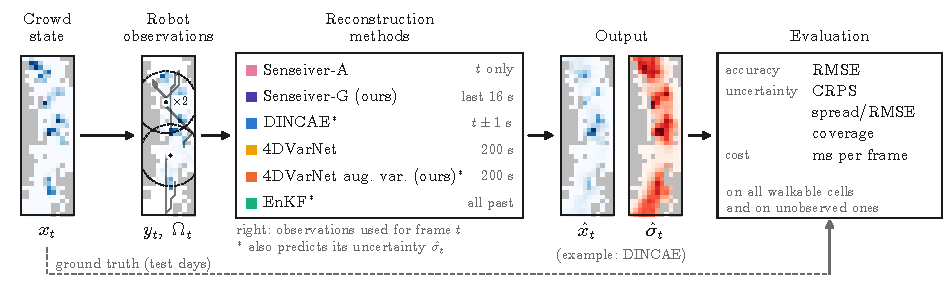
\includegraphics[width=\textwidth]{figures/pipeline.pdf}
	\caption{Overview of the study. The crowd state $x_t$ of a shopping-centre
	corridor is observed only partially, by three simulated robots ($y_t$, with
	observation mask $\Omega_t$). Six methods reconstruct the full state
	$\hat{x}_t$ from these observations; the right column of the method box gives
	the observations each method uses to reconstruct frame $t$. The three methods
	marked with an asterisk also predict their own uncertainty $\hat{\sigma}_t$.
	The reconstructions are scored against the ground truth of the held-out test
	days, on the walkable cells and separately on those that no robot observes. The thumbnails show the
	density channel of one test frame.}
	\label{fig:pipeline}
\end{figure}

%% ------------------------------------------------------------------
\subsection{Problem formulation}
\label{sec:problem}

The environment is a corridor discretised into a grid of $H \times W = 36
\times 12$ cells of $1\times1$\,m, observed once per second. The crowd state at
time $t$ is a four-channel field
\begin{equation}
	x_t = \big(\rho_t,\; v_{x,t},\; v_{y,t},\; \nu_t\big) \in \mathbb{R}^{4 \times H \times W},
	\label{eq:state}
\end{equation}
whose channels are, per cell, the pedestrian density $\rho$ (people per
m$^2$), the two components of the mean walking velocity $v_x, v_y$ (m/s,
along and across the corridor), and the velocity variance $\nu$ (m$^2$/s$^2$),
which measures the velocity dispersion of the tracking records contributing within one second to a cell (Section~\ref{sec:data}).
These are the macroscopic quantities referred to in
Section~\ref{sec:intro}: they describe the crowd without identifying any
individual. Only a fixed set $\mathcal{W}$ of cells is walkable; the others are
walls and the stalls lining the corridor (Section~\ref{sec:data}). Throughout
the thesis, array sizes are written in the order channels $\times$ frames
$\times$ rows $\times$ columns, leaving out the dimensions that an array does not
have, so that one state is $4 \times 36 \times 12$ and a window of 200 states
is $4 \times 200 \times 36 \times 12$.

At every second, a team of robots observes the cells near them. The set of
observed cells is described by a binary mask $\Omega_t \in \{0,1\}^{H \times
W}$, and the observation is the state on those cells corrupted by noise,
\begin{equation}
	y_t = \Omega_t \odot \big(x_t + \varepsilon_t\big), \qquad
	\varepsilon_{t} \sim \mathcal{N}\big(0,\, \mathrm{diag}(\sigma^2_{\mathrm{obs}})\big),
	\label{eq:obs}
\end{equation}
where $\odot$ is the element-wise product (applied to every channel) and
$\sigma_{\mathrm{obs}}$ holds one standard deviation per channel. The
four-dimensional noise distribution is applied independently at each cell and
second. A
reconstruction method maps a sequence of observations $(y_{t'}, \Omega_{t'})$ to an
estimate $\hat{x}_t$ of the full state; a probabilistic method also returns a
per-cell, per-channel standard deviation $\hat{\sigma}_t$. The predictive
distribution each method defines is stated with the method
(Section~\ref{sec:models}) and is what it is scored on
(Section~\ref{sec:eval}).
Methods differ in which observations they may use: a \emph{causal} method uses
only $t' \le t$, as an online estimator must, whereas a non-causal one also uses
observations after $t$. Of particular interest are the \emph{blind} cells
\begin{equation}
	\mathcal{B}_t = \{\, j \in \mathcal{W} : \Omega_{t,j} = 0 \,\},
	\label{eq:blind}
\end{equation}
the walkable cells that no robot observes at time $t$, where the state must be
inferred rather than read from an observation. Accuracy is scored on all
walkable cells and, separately, on the blind cells (Section~\ref{sec:eval}).

%% ------------------------------------------------------------------
\subsection{Research material: the ATC dataset and its preprocessing}
\label{sec:data}

This section describes the data and every step that turns it into the input of
the methods: which days are used and how they are split, how the tracking
records become a gridded state, and which cells of the grid are walkable
(Figure~\ref{fig:data_processing}).

\begin{figure}[htb]
	\centering
	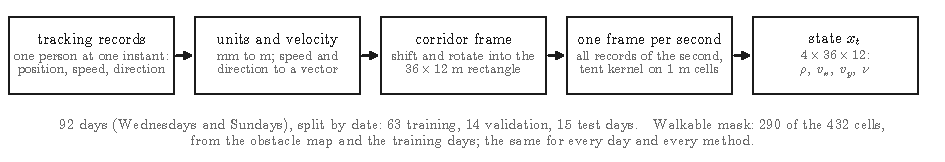
\includegraphics[width=\textwidth]{figures/data_processing.pdf}
	\caption{Preprocessing of the ATC dataset. Every tracking record is
	converted to metres and to a velocity vector and expressed in the coordinate
	frame of the corridor grid; all records of one second are then spread over
	the 1\,m cells, which gives one four-channel state per second.}
	\label{fig:data_processing}
\end{figure}

\subsubsection{Dataset and split}

The ground-truth crowd state is derived from the ATC pedestrian tracking dataset
\cite{brscic2013atc}, recorded in the Asia and Pacific Trade Center shopping centre in Osaka, Japan, by a
network of 3-D range sensors that track the positions of the pedestrians in the
covered area.
Each record gives the position and the velocity of one tracked person at one
time instant. The dataset covers Wednesdays and Sundays over about a year, 92
days in total, and all of them are used. The days are split chronologically,
never shuffled, so that no part of a day is seen from both sides of a split
boundary (Table~\ref{tab:split}); every split holds both Wednesdays and Sundays.
All model weights and training-derived statistics are fitted on the training
days, and checkpoints are selected on the validation days. The candidate
designs and configuration constants were chosen earlier in development on the
Sundays alone, with the same split boundaries, and are kept fixed for the
reported models (Section~\ref{sec:impl}). The evaluation reported in
Section~\ref{sec:results} uses those fixed choices. That earlier work also
inspected the seven Sunday test dates, so they were not untouched throughout
development.

\begin{table}[htb]
	\centering
	\caption{Chronological split of the 92 days of the ATC dataset: 31 Wednesdays
	and 32 Sundays for training, 7 and 7 for validation, 8 and 7 for testing.
	Frames are one second apart; a day covers about eleven hours.}
	\label{tab:split}
	\begin{tabular}{lrrl}
		\hline
		Split & Days & Frames & Date range \\
		\hline
		Training   & 63 & 2\,525\,609 & 24 Oct 2012 -- 9 Jun 2013 \\
		Validation & 14 &   535\,739  & 12 Jun 2013 -- 28 Jul 2013 \\
		Test       & 15 &   587\,227  & 7 Aug 2013 -- 29 Sep 2013 \\
		\hline
	\end{tabular}
\end{table}

\subsubsection{From tracking records to a gridded state}
\label{sec:gridding}
Each record of the dataset holds a timestamp, a person identifier, the
position of the person (two horizontal coordinates and the height) in millimetres, the speed in millimetres per second, the
direction of motion and the facing direction. The positions are converted to
metres, and the speed $s$ and the direction of motion $\alpha$ to a velocity
vector $u = s\,(\cos\alpha, \sin\alpha)$ in metres per second. The person
identifier, the height and the facing direction are not used: the state is a
macroscopic field, and the identity of the individuals plays no role in it. No
record is removed.

A $36 \times 12$\,m rectangle is placed along the main corridor of the tracked
area and rotated to align with it (Figure~\ref{fig:study_area}a): its origin is
at $(38.28, -15.81)$\,m in the coordinates of the dataset and it is rotated by
$2.565$\,rad. The positions and the velocity vectors are expressed in the
frame of this rectangle, so that $v_x$
points along the corridor and $v_y$ across it. For each one-second frame, every
tracked position $p$ recorded within that second is spread over the grid with a
bilinear (tent) kernel $k(p, c_j) = \prod_{d} \max(0, 1 - |p_d - c_{j,d}|)$,
where $c_j$ is the centre of cell $j$ in grid coordinates. With $n$ the number
of distinct sampling timestamps within the second, the channels of cell $j$ are
\begin{equation}
	\begin{aligned}
	\rho_j &= \frac{1}{n} \sum_{p} k(p, c_j), \qquad
	(v_x, v_y)_j = \frac{1}{n \rho_j} \sum_{p} k(p, c_j)\, u_p, \\
	\nu_j &= \frac{m_j}{m_j - 1}\,\frac{1}{n \rho_j} \sum_{p} k(p, c_j)\, \|u_p - \bar{u}_j\|^2,
	\end{aligned}
	\label{eq:gridding}
\end{equation}
where $u_p$ is the velocity of record $p$, $\bar{u}_j = (v_x, v_y)_j$, and
$m_j$ is the number of records with non-zero weight in the cell, including
repeated records of the same pedestrian within the second. Thus $\nu_j$
describes the dispersion of those contributing velocity records; the velocity
and the velocity variance are set to zero in empty cells, and the variance also
where fewer than two records contribute. Because a cell is 1\,m$^2$, $\rho$ is
directly a density in people per m$^2$. The result is one $4 \times 36 \times
12$ state per second (Figure~\ref{fig:study_area}c--f).

\paragraph{Recording gaps.}
The frames are formed from the sequence of the tracker's sampling timestamps:
timestamps are collected into a frame until one reaches the frame's end time,
and the end time then advances by one second. When the recording pauses, this
windowing does not skip the missing seconds. After the pause it emits one frame
per sampling timestamp until its end time has caught up, so each of these frames
holds a single snapshot taken after the pause, under a time label that lags the
real time. A frame is flagged when any of its timestamps lies outside its
labelled second by more than 0.1\,s. Flagged frames make up 0.63\% of all
frames and occur on 27 of the 92 days, mostly in a few long pauses of up to
76\,min. They are kept in the data and in training, but not scored: every
aligned 200-frame block (the 4DVarNet windows) that contains a flagged frame is
excluded, together with the following block, for every method, both when
checkpoints are selected on the validation days and in the test scores, so
that methods that carry information across frames are not scored while they
recover. This removes 2.9\% of the validation frames and 1.5\% of the test
frames, on four of the test days. The residuals that form the EnKF's process
noise (Section~\ref{sec:enkf}) are likewise drawn from the remaining training
frames.

\subsubsection{Walkable cells}
A cell is treated as a wall if at least half of its area is occupied by
obstacles in the map of the ATC environment, which includes the stalls and
pillars inside the corridor. A cell is additionally required to have been
walked: its density must exceed 0.5 in at least one frame of the training days,
which removes cells outside the corridor walls that receive density only
through the kernel's spill-over. Of the remaining cells, the largest connected
component is kept, so that every walkable cell is reachable by a robot. This
yields $|\mathcal{W}| = 290$ walkable cells out of 432 (Figure~\ref{fig:study_area}b);
the mask is the same for every day and every method. The networks reconstruct,
and are trained on, the whole $36 \times 12$ rectangle: the supervised
reconstruction losses do not use the walkable mask. The robots navigate only
on $\mathcal{W}$, and reconstruction scores exclude non-walkable cells.
The observation footprint is
defined by range and line of sight and is not intersected with the mask
afterwards.

\begin{figure}[htb]
	\centering
	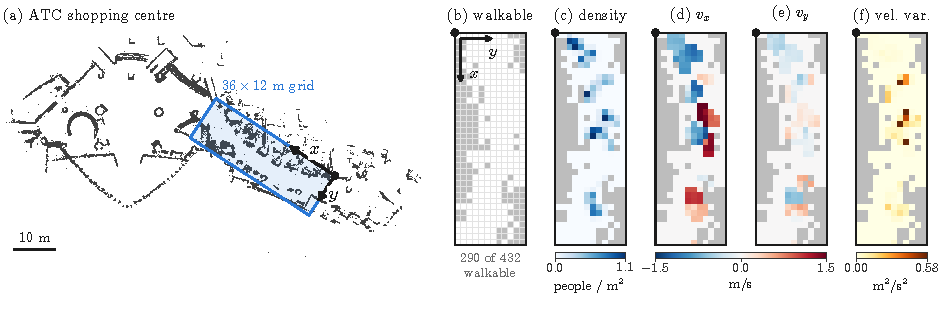
\includegraphics[width=\textwidth]{figures/study_area.pdf}
	\caption{The study area. (a) Obstacle map of the ATC shopping centre with the
	$36 \times 12$\,m corridor grid; the black dot marks the grid origin, also
	marked in (b)--(f), and the arrows the grid axes $x$ (along the corridor) and
	$y$ (across it), drawn again in (b). (b) The 290 walkable cells (white); grey
	cells are walls and stalls. (c)--(f) The four channels of the state at one
	second of a test day: density, the velocity components $v_x$ and $v_y$
	(positive along the arrows $x$ and $y$), and the velocity variance.}
	\label{fig:study_area}
\end{figure}

%% ------------------------------------------------------------------
\subsection{Simulated multi-robot partial observations}
\label{sec:obs}

The robots and their observations are simulated: an observation is the
ground-truth state on the observed cells plus Gaussian noise of an assumed size
(Eq.~\eqref{eq:obs}). Real on-board sensing would add occlusion by
pedestrians, detection errors and errors in the robots' own localisation, so
the results describe the methods under idealised observations; how they
transfer to real robot deployments is not tested in this thesis.

The partial observations are produced by simulating a team of three mobile
robots in the corridor. Each robot starts on a random
walkable cell, is given a random walkable goal, and follows the shortest
obstacle-free path to it, computed with the A$^*$ search algorithm on the 8-connected grid of
walkable cells; it moves one cell per second and draws a new goal on arrival.
The robots do not react to the crowd, so the observation pattern is independent
of the state being estimated.

A cell is observed by a robot at a given second if the Euclidean distance
between their cell centres is at most 7 cells and the straight line between the
two centres does not pass through a wall cell, using the same wall definition as
the walkable mask (Figure~\ref{fig:observation}a). The line is tested at steps
of 0.1 cell, and only the cells between the two end cells can block it, so a
wall cell itself is observed when no other wall cell lies in between. Each
robot first moves and then observes, once per second. The mask $\Omega_t$ is the union
over the three robots, and every observed cell yields all four channels. The
observation noise in Eq.~\eqref{eq:obs} has standard deviations
$\sigma_{\mathrm{obs}} = (0.057,\ 0.315,\ 0.086,\ 0.0064)$ for $(\rho, v_x, v_y,
\nu)$. They are set to a
quarter of a robust estimate of each channel's natural variability (1.4826 times
the median absolute deviation over occupied cells), on the assumption that a
sensor is more precise than the fluctuations of the field itself.

The routes are generated from a random seed derived from the date, so that every
day has its own routes and every method sees exactly the same observations of a
given day. The noise is drawn from a second random stream, also seeded by the
date, and the noisy values are not clipped, so an observed density can be
slightly negative. The observations of a day, routes and noise, are generated
once: the training days carry the same observations in every epoch, and the
noise is not redrawn. With a sensing radius of 7 cells, on average 56\% of the walkable
cells are observed at a given second (Figure~\ref{fig:observation}c); the
remaining 44\% are the blind cells. Since the
robots keep moving, blindness is mostly short-lived: on a representative test
day, 68\% of the blind cells were observed within the preceding 15\,s and 99\%
within the preceding 200\,s (Figure~\ref{fig:observation}d). This is what makes
methods that accumulate observations over time worth considering, and it bounds
the useful length of their temporal context.

\begin{figure}[htb]
	\centering
	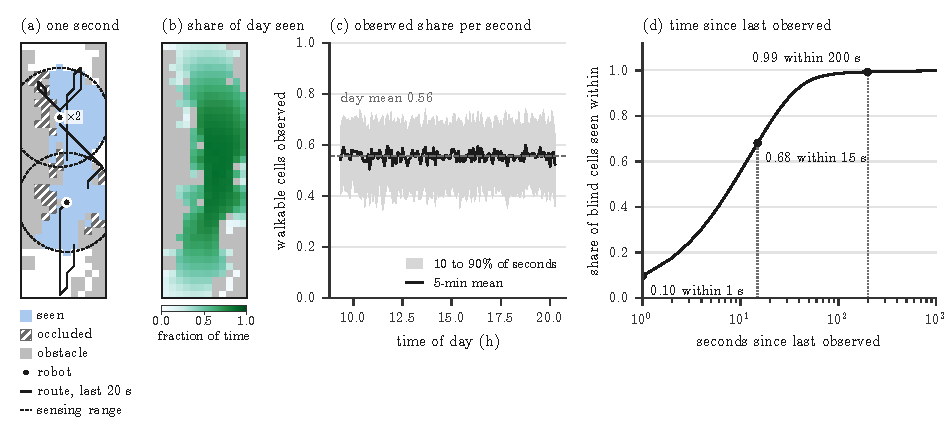
\includegraphics[width=\textwidth]{figures/observation.pdf}
	\caption{The simulated observations, on the test day of 11 August 2013.
	(a) One second: the robots (dots; two of the three share a cell at this
	second), their routes over the last 20\,s, the 7-cell sensing radius
	(dashed), the walkable cells they observe (blue) and the cells within range
	that obstacles hide from them (hatched). (b) Fraction of the day during which
	each cell is observed. (c) Fraction of the walkable cells observed at each
	second: 10--90\% range over the seconds of each five-minute block (grey) and
	its mean (black). (d) For the blind cells, the distribution of the time since
	the cell was last observed.}
	\label{fig:observation}
\end{figure}

%% ------------------------------------------------------------------
\subsection{Reconstruction methods}
\label{sec:models}

Six methods are compared (Table~\ref{tab:methods}). Four are existing methods,
reproduced for this problem: Senseiver \cite{santos2023senseiver}, labelled
Senseiver\nobreakdash-A after its abstract latent array, DINCAE
\cite{barth2022dincae2}, 4DVarNet \cite{fablet2020fourdvarnet}, and a localised
EnKF \cite{roth2017enkf}. Two are
extensions proposed in this thesis: Senseiver\nobreakdash-G, a Senseiver whose latent array
is the grid itself and which reads a window of past observations, and the
4DVarNet with an augmented variance, an uncertainty-aware 4DVarNet, called the
augmented 4DVarNet in the text and labelled ``4DVarNet aug.\ var.'' in tables
and figures. The methods differ in which observations
they use to reconstruct a frame (Figure~\ref{fig:time_windows}), in whether they
are causal, and in whether they predict their own uncertainty.

\begin{table}[htb]
	\centering
	\caption{The six reconstruction methods. Observations used to reconstruct
	frame $t$; whether the method is causal; and whether it predicts an
	uncertainty $\hat{\sigma}$, and from what.}
	\label{tab:methods}
	\begin{tabular}{llcc}
		\hline
		Method & Observations & Causal & $\hat{\sigma}$ \\
		\hline
		Senseiver\nobreakdash-A                  & $t$                   & yes & --                 \\
		Senseiver\nobreakdash-G (ours)           & $t-15, \dots, t$      & yes & --                 \\
		DINCAE                       & $t-1, t, t+1$         & no  & network output     \\
		4DVarNet                     & 200-s window          & no  & --                 \\
		4DVarNet aug.\ var.\ (ours) & 200-s window          & no  & iterated with $x$  \\
		EnKF                         & all $t' \le t$        & yes & ensemble spread    \\
		\hline
	\end{tabular}
\end{table}

\begin{figure}[htb]
	\centering
	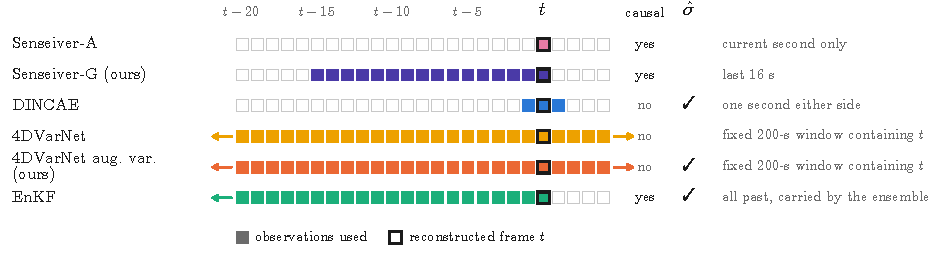
\includegraphics[width=\textwidth]{figures/time_windows.pdf}
	\caption{The observations each method uses to reconstruct frame $t$ (filled
	squares; the framed square is frame $t$ itself). Arrows mean the window
	extends beyond the part drawn. 4DVarNet reconstructs fixed, non-overlapping
	200-second windows, so frame $t$ is reconstructed from the whole window that
	contains it. Its initial field may retain observations from earlier in the
	day. The EnKF carries past observations through its ensemble.
	The two columns after the squares state whether the method is causal and whether it
	predicts its uncertainty $\hat{\sigma}$.}
	\label{fig:time_windows}
\end{figure}

The five observation-conditioned reconstruction models are trained on
the 63 training days with the gridded state as target. Ground truth enters
their supervised reconstruction losses; inference uses observations and fixed
position and time features. PedPred3, the EnKF's forecast model, is
trained separately to predict future ground-truth states from past
ground-truth states. Reconstruction checkpoints are selected by validation
reconstruction error, while PedPred3 is selected by validation forecast loss
(Section~\ref{sec:impl}).

Table~\ref{tab:io} summarises, before the methods are described one by one,
what each of them receives and returns when it reconstructs. The methods differ
not only in their network but in the form of their input: Senseiver reads a
set of tokens, one per observed cell, whose number changes from second to
second; DINCAE reads images on the grid, with zeros and a mask where nothing
was observed; the two 4DVarNet models read a whole 200-second window at once; and the EnKF
receives the observations one second at a time and carries everything else in
its ensemble.

\begin{table}[htb]
	\centering
	\caption{Inputs and outputs of each method for one reconstruction. $N_s$ is
	the number of cells in the robots' observation footprint at one second,
	which is not restricted to the walkable cells: on the test days it averages
	about 200, of which about 160 are walkable (the 56\% of
	Section~\ref{sec:obs} counts only the 290 walkable cells). $N_w \le 16 N_s$ is
	the number of tokens in the 16-second window of Senseiver\nobreakdash-G, the sum of $N_s$
	over its frames. Sizes are channels $\times$ frames $\times$ rows $\times$
	columns, or tokens $\times$ values per token. All outputs cover
	the whole $36 \times 12$ grid; the scores use only the walkable cells.}
	\label{tab:io}
	\small
	\begin{tabular}{L{0.15\textwidth}L{0.42\textwidth}L{0.34\textwidth}}
		\hline
		Method & Input & Output \\
		\hline
		Senseiver\nobreakdash-A & $N_s \times 68$: one token per observed cell of frame $t$, \mbox{$4 + 64 = 68$} values (observation, position encoding) & $\hat{x}_t$: $4 \times 36 \times 12$ \\
		Senseiver\nobreakdash-G & $N_w \times 77$: one token per observed cell of each of the frames $t-15, \dots, t$, \mbox{$4 + 64 + 8 + 1 = 77$} values (with time offset) & $\hat{x}_t$: $4 \times 36 \times 12$ \\
		DINCAE & one image of $30 \times 36 \times 12$: for frames $t-1, t, t+1$ and each of the 4 channels, the observed normalised residual and the mask (24), plus 2 coordinates and 4 time-of-day and day-of-week encodings & $\hat{x}_t$ and $\hat{\sigma}_t$: $4 \times 36 \times 12$ each \\
		4DVarNet & $y$, $\Omega$ and the initial field $x^{(0)}$ of one window, each \mbox{$4 \times 200 \times 36 \times 12$} & $\hat{x}$ for the whole window: \mbox{$4 \times 200 \times 36 \times 12$} \\
		4DVarNet aug.\ var. & as 4DVarNet & $\hat{x}$ and $\hat{\sigma}$ for the whole window: \mbox{$4 \times 200 \times 36 \times 12$} each \\
		EnKF & at each second, the $4 N_s$ observed values; internally 100 members of $4 \times 36 \times 12$, each forecast from its last five analyses & ensemble mean $\hat{x}_t$ and standard deviation $\hat{\sigma}_t$: $4 \times 36 \times 12$ each \\
		\hline
	\end{tabular}
\end{table}

\subsubsection{Senseiver-A}
\label{sec:senseiver_a}

Senseiver \cite{santos2023senseiver} treats the observations as an unordered
set of tokens and compresses them into a fixed-size latent array with
attention, following Perceiver IO \cite{jaegle2021perceiver}
(Figure~\ref{fig:senseiver}a). Every observed cell $i$ at time $t$ becomes one
token
\begin{equation}
	e_i = \big[\, \tilde{y}_i,\; \mathrm{PE}(\chi_i) \,\big] \in \mathbb{R}^{4+64},
	\label{eq:sv_token}
\end{equation}
where $\tilde{y}_i$ holds the four observed values, standardised with a
per-channel mean and standard deviation computed over the observed cells of the
training frames only -- that is, over the noisy readings that actually reach the
encoder, not over the complete fields -- and
$\mathrm{PE}(\chi_i)$ is a sinusoidal encoding of the cell position $\chi_i$, as
in the reference implementation,
\begin{equation}
	\begin{aligned}
	\mathrm{PE}(\chi) &= \Big[\, \sin\!\big(\pi \omega^{(1)}_k \chi^{(1)}\big),\;
	\sin\!\big(\pi \omega^{(2)}_k \chi^{(2)}\big),\; \\
	&\qquad\; \cos\!\big(\pi \omega^{(1)}_k \chi^{(1)}\big),\;
	\cos\!\big(\pi \omega^{(2)}_k \chi^{(2)}\big) \,\Big]_{k = 1, \dots, 16}, \\
	\omega^{(m)}_k &= 1 + \frac{k - 1}{15} \Big( \frac{N_m}{2} - 1 \Big),
	\end{aligned}
	\label{eq:sv_pe}
\end{equation}
where $\chi^{(1)}$ and $\chi^{(2)}$ are the row and the column of the cell,
mapped linearly to $[-1, 1]$ (the first cell to $-1$, the last to $1$), and
$N_1 = 36$ and $N_2 = 12$ are the numbers of cells along the corridor and
across it: 16 frequencies per coordinate, spaced linearly from 1 to half the
number of cells (18 along the corridor, 6 across it). A linear layer maps the
tokens to 32 channels, $e'_i = W_e e_i + b_e$.

The encoder holds an array of 64 learned latent vectors of 32 channels,
initialised from a normal distribution with standard deviation 0.02. It
consists of three blocks, each a cross-attention in which the latents are the
queries and the tokens the keys and values, followed by three self-attention
layers among the latents; the first block has its own weights and the second and
third share one set. Each block thus re-reads the observations. The decoder
reconstructs the field cell by cell: the query of cell $j$ is its position
encoding $\mathrm{PE}(\chi_j)$ concatenated with a learned vector of 32 values
that is shared by all cells (initialised like the latents), and a
cross-attention from these 432 queries to the latent array, followed by a linear
layer, returns the four channels of every cell. The model accepts any number of
observed cells: within a batch the token sets are padded to the largest count in
that batch, and a key-padding mask excludes the padding slots from every
attention, so what the model returns does not depend on how much padding its
batch-mates required.

Figure~\ref{fig:attention_block} shows what happens inside one encoder block.
Every attention layer has two halves, the attention itself and a two-layer
perceptron with a GELU non-linearity; each half is preceded by a layer
normalisation (in the cross-attention, one for the latents and one for the
sensor tokens) and wrapped in a residual connection, that is, its output is
added to its input (Section~\ref{sec:bg_nn}). In the cross-attention layer, the latents are the queries
and the sensor tokens the keys and values, so every latent collects information
from all observations; the number of latents is unchanged. In the three
self-attention layers that follow, queries, keys and values are all the
latents, so the latents exchange information with each other. The output of
one block is the latent array that enters the next block, which attends to the
same sensor tokens again. Written out, with $z$ the latent array and $e'$ the
projected tokens, a cross-attention layer and a self-attention layer update $z$
as
\begin{equation}
	\begin{aligned}
	\text{cross-attention:}\quad
	z &\leftarrow z + \mathrm{MHA}\big(\mathrm{LN}_{q}(z),\, \mathrm{LN}_{e}(e'),\, \mathrm{LN}_{e}(e')\big), \\
	z &\leftarrow z + \mathrm{MLP}\big(\mathrm{LN}(z)\big), \\
	\text{self-attention:}\quad
	z &\leftarrow z + \mathrm{MHA}\big(\mathrm{LN}(z),\, \mathrm{LN}(z),\, \mathrm{LN}(z)\big), \\
	z &\leftarrow z + \mathrm{MLP}\big(\mathrm{LN}(z)\big),
	\end{aligned}
	\label{eq:sv_layers}
\end{equation}
with $\mathrm{MHA}$ and $\mathrm{LN}$ of Eqs.~\eqref{eq:bg_mha} and
\eqref{eq:bg_ln}, $\mathrm{MLP}(a) = W_2\, \mathrm{GELU}(W_1 a + b_1) + b_2$,
and every $\mathrm{LN}$, $\mathrm{MHA}$ and $\mathrm{MLP}$ with its own weights.
A block is one cross-attention layer followed by three
self-attention layers, and the encoder computes
$z = \mathrm{Block}_2\big(\mathrm{Block}_2\big(\mathrm{Block}_1(z^{(0)}, e'), e'\big), e'\big)$
from the learned latent array $z^{(0)}$, where $\mathrm{Block}_2$ is the block
whose weights the second and third blocks share. The decoder forms the query
$q_j = W_q\, [\mathrm{PE}(\chi_j), w] + b_q$ of every cell $j$ from the shared
learned vector $w$, applies one cross-attention layer of
Eq.~\eqref{eq:sv_layers} to it, with $q_j$ in place of $z$ and the latent array
$z$ as keys and values, and returns $\hat{x}_j = W_o\, q_j + b_o$.
Table~\ref{tab:arch_senseiver} lists the sizes
of all components. Senseiver\nobreakdash-A follows the reference architecture with these
sizes. It is trained on the crowd problem with the reference loss, the sum of squared errors over all cells and
channels in physical units, and it reconstructs every frame from that frame's
observations only.

\begin{figure}[htb]
	\centering
	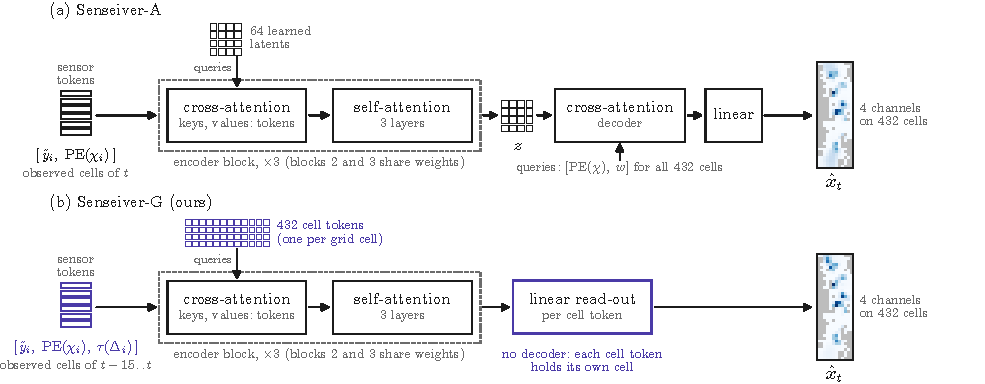
\includegraphics[width=\textwidth]{figures/senseiver.pdf}
	\caption{(a) Senseiver\nobreakdash-A. Each observed cell becomes a token of observed
	values and position encoding; three encoder blocks (cross-attention from 64
	learned latents to the tokens, then three self-attention layers) produce a
	latent array $z$, from which a cross-attention decoder, queried with the
	positions of all 432 cells, reconstructs the field. (b) Senseiver\nobreakdash-G (ours).
	The latent array is the grid: one token per cell, whose initial value is a
	learned projection of the cell's position encoding. The decoder is replaced
	by a linear read-out of each cell's own token, and the sensor tokens of the
	last 16\,s carry their time offset $\Delta_i$. Parts changed in (b) are
	drawn in colour. The thumbnails are each model's density reconstruction of
	one test frame.}
	\label{fig:senseiver}
\end{figure}

\begin{figure}[htb]
	\centering
	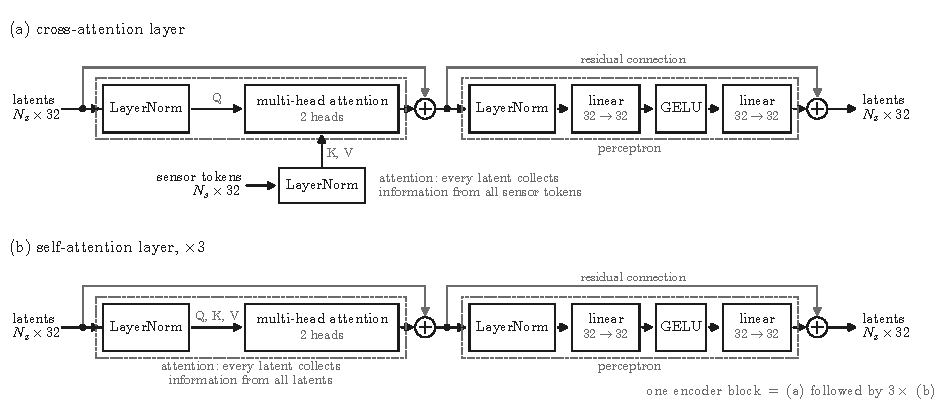
\includegraphics[width=\textwidth]{figures/attention_block.pdf}
	\caption{Inside one encoder block of the Senseiver models; the block is the
	same in Senseiver\nobreakdash-A ($N_z = 64$ latents) and Senseiver\nobreakdash-G ($N_z = 432$ cell
	tokens), and $N_s$ is the number of sensor tokens. (a) The cross-attention
	layer: the latents are the queries (Q) and the sensor tokens the keys and
	values (K, V) of a multi-head attention, followed by a two-layer perceptron.
	(b) A self-attention layer, in which queries, keys and values are all the
	latents; three of these follow the cross-attention layer. Both halves of
	every layer start with a layer normalisation, and their output is added to
	their input (residual connection). The encoder runs three such blocks one
	after the other.}
	\label{fig:attention_block}
\end{figure}

\begin{table}[htb]
	\centering
	\caption{Architecture of the two Senseiver models. ``Linear $a \to b$'' is a
	fully connected layer from $a$ to $b$ channels; all attention layers work
	with 32 channels.}
	\label{tab:arch_senseiver}
	\small
	\begin{tabular}{L{0.2\textwidth}L{0.35\textwidth}L{0.35\textwidth}}
		\hline
		Component & Senseiver\nobreakdash-A & Senseiver\nobreakdash-G (ours) \\
		\hline
		Sensor token & 4 values + 64 position encoding = 68 & 4 values + 64 position encoding + 8 time embedding + 1 time scalar = 77 \\
		Token projection & linear $68 \to 32$ & linear $77 \to 32$ \\
		Latent array (queries) & 64 learned vectors of 32 channels & 432 cell tokens: linear $64 \to 32$ of each cell's position encoding \\
		Encoder block ($\times 3$; blocks 2 and 3 share weights) & \multicolumn{2}{L{0.7\textwidth}}{cross-attention to the tokens (2 heads), then 3 self-attention layers (2 heads); each followed by a perceptron $32 \to 32 \to 32$} \\
		Read-out & query: linear $96 \to 32$ of [64 position encoding, 32 learned]; cross-attention to the latents (1 head); linear $32 \to 4$ & linear $32 \to 4$ applied to each cell token \\
		\hline
	\end{tabular}
\end{table}

\subsubsection{Senseiver-G: a grid latent with a temporal window (ours)}
\label{sec:senseiver_g}

Senseiver\nobreakdash-A has two properties that do not suit this problem. First, its
latent array is abstract: 64 latent vectors, none tied to a location, must
store a field of 432 cells, and every cell's value must then be retrieved from
them by the decoder. Second, it sees only the current second, although the
robots observed 68\% of the currently blind cells within the last 15\,s
(Section~\ref{sec:obs}). Senseiver\nobreakdash-G changes both (Figure~\ref{fig:senseiver}b).

\paragraph{Grid latent and direct read-out.}
The latent array is made the grid itself: it holds one token per cell, 432 in
all, and the initial token of cell $j$ is a learned linear projection of its
position encoding, $z^{(0)}_j = A_z\, \mathrm{PE}(\chi_j) + b_z$. The queries
therefore carry the location of the cell, but no data: they are the same for
every frame. The encoder is otherwise unchanged, with the same three blocks of
cross-attention and self-attention. Because every cell now has its own token
after the encoder, no decoder is needed to retrieve a cell's value from an
abstract latent: a single linear layer, shared by all cells, maps each cell's
token to its four channels. Self-attention among the 432 cell tokens lets
information from observed cells reach the blind ones. Letting every output
location act as a query that attends to the observations is also the mechanism
of attentive neural processes \cite{kim2019anp}, in which each target location
cross-attends to the observed context points.

\paragraph{Temporal window.}
The tokens are drawn from the observations of the last $L = 16$ seconds,
$t-15, \dots, t$, rather than from frame $t$ alone; at the start of a day, the
window is shorter. A cell observed in several of these seconds contributes
several tokens with the same position encoding. Each token is extended with an
encoding of its time offset $\Delta_i = t - t'_i \in \{0, \dots, 15\}$,
\begin{equation}
	e_i = \big[\, \tilde{y}_i,\; \mathrm{PE}(\chi_i),\; \tau(\Delta_i) \,\big],
	\qquad \tau(\Delta) = \big[\, E_{\Delta},\; \Delta / L \,\big] \in \mathbb{R}^{8+1},
	\label{eq:sv_token_g}
\end{equation}
where $E \in \mathbb{R}^{L \times 8}$ is a learned embedding table, one learned
vector $E_{\Delta}$ of 8 values for each offset, and the
scalar $\Delta / L$ gives the model the order of the offsets. A window of
16\,s covers the time within which about two thirds of the blind cells have
been observed at least once (Section~\ref{sec:obs}); the window length was
selected during the Sunday-only development among 1, 4, 8 and 16\,s
(Section~\ref{sec:impl}). The model remains causal. It is trained with the same
loss as Senseiver\nobreakdash-A. The use of the recent measurements of moving sensors
follows the motivation of the mobile-sensor SHRED \cite{ebers2024mobileshred};
here the past observations enter as additional tokens with their time offsets,
so that their varying number needs no fixed input layout.

Each reconstruction is independent of the previous one. The token set is built
afresh from the window that ends at the frame being reconstructed, and the cell
tokens start from $z^{(0)}$, which is a learned initialisation shared by every
frame rather than a state carried over from the frame before. All of the
model's temporal information is therefore in the window: the grid latent is not
a recurrent memory, as the hidden state of a convolutional LSTM or the ensemble
of a filter is, and nothing reaches frame $t$ from further back than
$t - 15$.

In summary, Senseiver\nobreakdash-G reconstructs frame $t$ as
\begin{equation}
	\begin{aligned}
	e'_i &= W_e \big[\, \tilde{y}_i,\; \mathrm{PE}(\chi_i),\; E_{\Delta_i},\; \Delta_i / L \,\big] + b_e, \\
	z^{(0)}_j &= A_z\, \mathrm{PE}(\chi_j) + b_z, \\
	z &= \mathrm{Block}_2\big(\mathrm{Block}_2\big(\mathrm{Block}_1(z^{(0)}, e'), e'\big), e'\big), \\
	\hat{x}_{t,j} &= W_r\, z_j + b_r,
	\end{aligned}
	\label{eq:sv_g}
\end{equation}
for every token $i$ of frames $t-15, \dots, t$ and every cell $j = 1, \dots, 432$,
with the blocks of Eq.~\eqref{eq:sv_layers}, $W_e$ mapping
$77 \to 32$ channels, $A_z$ mapping $64 \to 32$ and $W_r$ mapping $32 \to 4$.
The read-out returns the four channels in physical units; the observed values
enter standardised, and the output is not rescaled.

\subsubsection{DINCAE}
\label{sec:dincae}

DINCAE \cite{barth2020dincae1, barth2022dincae2} is a convolutional
encoder--decoder that reconstructs a gridded field and its error variance from
observations with gaps (Figure~\ref{fig:dincae}). The implementation follows
DINCAE~2.0 \cite{barth2022dincae2}; the adaptations to this problem are stated
below.

\paragraph{Input.}
Each channel is first transformed to a residual: it is reduced by its per-cell mean over
the training days and divided by one standard deviation per channel. The
per-cell mean is taken only over the frames in which the channel is defined at
that cell: all frames for density, the frames in which the cell is occupied for
the two velocity components, and the frames with a non-zero velocity variance
for $\nu$. The standard deviation pools the deviations from these means over
all walkable cells and over the frames in which the channel is defined. For input encoding, the error variance in this normalised space is
set to one, following the reference implementation. This does not change the
simulated observation noise of Section~\ref{sec:obs}. The information-form pair,
residual divided by error variance and inverse error variance, therefore
becomes the observed normalised residual and the mask. These two slices are provided for frames
$t-1$, $t$ and $t+1$, together with the two cell coordinates and sine--cosine
encodings of the daily and weekly cycles, for 30 input channels.

\paragraph{Network.}
The network is a U-Net with three levels of $3 \times 3$ convolutions with
32, 64 and 96 filters and $2 \times 2$ mean pooling, which reduces the $36
\times 12$ grid to $18 \times 6$, $9 \times 3$ and $5 \times 2$; odd sizes are
handled by ceiling pooling and by cropping after upsampling. Following DINCAE~2.0,
the skip connections at the two inner levels are additive rather than
concatenative, and a second network of the same structure refines the output:
it receives the input together with the first network's output. For every
channel, each network returns two values per cell, which are converted into a
mean $\mu$ and a variance $\varsigma^2$ in the normalised space, through the
information-form parametrisation of the reference implementation (the network
predicts $\mu/\varsigma^2$ and $\log(1/\varsigma^2)$, and the precision is bounded so that $\varsigma^2
\in [e^{-10}, 10^{3}]$). Table~\ref{tab:arch_dincae} lists the layers.

\begin{table}[htb]
	\centering
	\caption{Layers of the DINCAE network. All convolutions are $3 \times 3$;
	pooling is $2 \times 2$ mean pooling and upsampling is nearest-neighbour by
	a factor of 2, cropped to the size of the corresponding encoder level. The
	refinement network is identical, except that its input has 38 channels (the
	30 input channels and the 8 outputs of the first network).}
	\label{tab:arch_dincae}
	\small
	\begin{tabular}{lL{0.5\textwidth}ll}
		\hline
		Level & Operation & Channels & Output size \\
		\hline
		Encoder 1 & convolution, ReLU, pooling & $30 \to 32$ & $18 \times 6$ \\
		Encoder 2 & convolution, ReLU, pooling & $32 \to 64$ & $9 \times 3$ \\
		Encoder 3 & convolution, ReLU, pooling & $64 \to 96$ & $5 \times 2$ \\
		Decoder 3 & upsampling, convolution, ReLU; added to the input of encoder 3 & $96 \to 64$ & $9 \times 3$ \\
		Decoder 2 & upsampling, convolution, ReLU; added to the input of encoder 2 & $64 \to 32$ & $18 \times 6$ \\
		Decoder 1 & upsampling, convolution (no activation) & $32 \to 8$ & $36 \times 12$ \\
		\hline
	\end{tabular}
\end{table}

\paragraph{Training.}
The model is trained with a Gaussian negative log-likelihood, implemented as
\begin{equation}
	\mathcal{L}_{\mathrm{NLL}} = \sum_{\ell=1}^{2} w_\ell \sum_{c=1}^{4} \frac{1}{N_c} \sum_{i}
	\left[ \frac{(\xi_{c,i} - \mu_{\ell,c,i})^2}{\varsigma_{\ell,c,i}^2} + \log \varsigma_{\ell,c,i}^2 \right],
	\qquad (w_1, w_2) = (0.3,\ 0.7),
	\label{eq:nll}
\end{equation}
where $\ell$ indexes the two network outputs, $c$ the four channels, $i$ the
cells of a training batch, $N_c$ their number, and $\xi_{c,i}$ is the true
normalised residual. Each channel is averaged separately and the four averages
are summed, and the factor $\tfrac{1}{2}$ of the negative log-density of
Eq.~\eqref{eq:bg_nll} is omitted. The reference implementation trains against observed
values withheld from the input, because no ground truth is available for
satellite data; since the ground truth is available here, the loss is computed
against the true state on every cell, as for the other learned models.

\paragraph{Output.}
Normalisation is undone using the training mean and channel
standard deviation. For every channel, this gives a Gaussian
predictive distribution in physical units, whose mean is the point estimate
and whose standard deviation is reported as $\hat{\sigma}$.

\begin{figure}[htb]
	\centering
	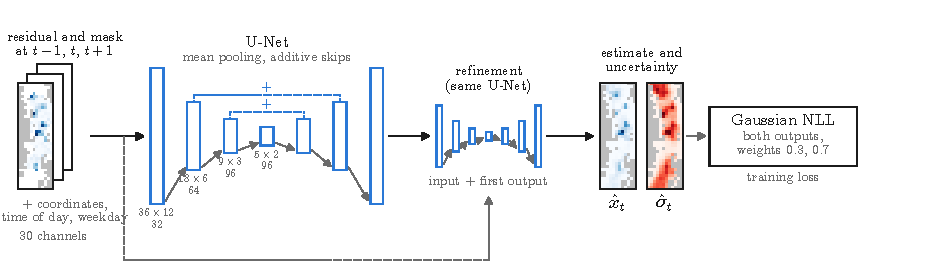
\includegraphics[width=\textwidth]{figures/dincae.pdf}
	\caption{DINCAE. The input holds, for frames $t-1$, $t$ and $t+1$, the
	observed normalised residual and the mask (both zero where unobserved),
	together with the cell
	coordinates and the time of day and week (30 channels). A U-Net with mean
	pooling and additive skips (sizes and filter counts below each level) is
	followed by a refinement U-Net of the same structure, which also receives the
	input. The final output is a point estimate $\hat{x}_t$ and a predictive
standard deviation $\hat{\sigma}_t$ per cell and channel; the point estimate is
the predictive mean.
Training uses a Gaussian negative log-likelihood in the normalised space
for both network outputs.}
	\label{fig:dincae}
\end{figure}

\subsubsection{4DVarNet}
\label{sec:varnet}

4DVarNet \cite{fablet2020fourdvarnet, fablet2021james} reconstructs a window of
$T$ consecutive states $x = (x_1, \dots, x_T)$ through learned updates guided
by a variational cost. The cost is
\begin{equation}
	J(x) = \alpha_{\mathrm{obs}}^2 \,\big\| (x - y) \odot \Omega \big\|^2_{W_{\mathrm{obs}}}
	     + \alpha_{\mathrm{reg}}^2 \,\big\| x - \Phi(x) \big\|^2_{W_{\mathrm{reg}}},
	\label{eq:varcost}
\end{equation}
where the first term measures the fit to the observations and the second the
consistency of the state with a learned prior $\Phi$; $\alpha_{\mathrm{obs}},
\alpha_{\mathrm{reg}}$ are learned scalars and $W_{\mathrm{obs}},
W_{\mathrm{reg}}$ learned per-channel coefficients. Each squared norm
sums squared residuals over the batch, time and grid, weights each physical
channel by its squared coefficient, and divides by the number of points per
channel.

\paragraph{Prior.}
$\Phi$ is the two-scale Gibbs-energy neural network (GENN) of
\citeauthor{fablet2020fourdvarnet} \cite{fablet2020fourdvarnet}. Each scale
applies a 3-D convolution over time, row and column with a $3 \times 3 \times
3$ kernel, from the 4 channels of the state to 96 channels, whose central tap
(the kernel weight at the position being computed) is set to zero, followed by a ReLU and two point-wise ($1 \times 1 \times 1$)
convolutions, $96 \to 96$ with a ReLU and $96 \to 4$. The coarse scale operates
on the state after $2 \times 2$ mean pooling in space, and its output is brought
back to the full grid by a transposed convolution and added to that of the fine
scale.

The prior maps a state window to another window of the same shape.
The zeroed central tap makes each branch independent of the input at the
point it predicts: the masked convolution excludes that space-time position,
and the subsequent layers are point-wise. Spatial pooling and upsampling are applied independently at each
time: the channel and time axes are exchanged before time is folded into the
batch axis, so the transposed convolution mixes the four physical channels of
one frame. Its kernel and stride are both 2, so each fine-grid output uses one
coarse output, which excludes its own pooled space-time input. The two-scale
$\Phi$ therefore also excludes dependence on the input at its own space-time
position and cannot represent the identity map (Figure~\ref{fig:genn}).

\begin{figure}[htb]
	\centering
	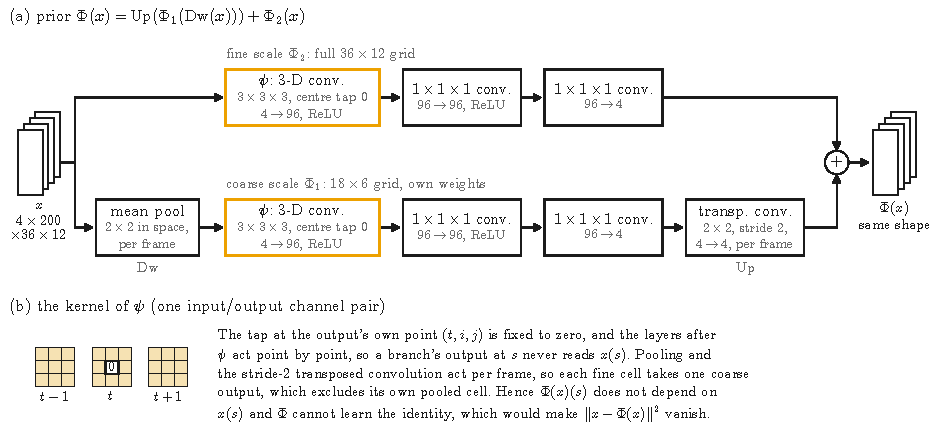
\includegraphics[width=\textwidth]{figures/genn.pdf}
	\caption{The prior $\Phi$ of 4DVarNet, a two-scale GENN
	\cite{fablet2020fourdvarnet}. (a) The fine branch $\Phi_2$ works on the full
	grid; the coarse branch $\Phi_1$, with its own weights, works on the state after
	$2 \times 2$ mean pooling in space and is brought back to the full grid by a
	transposed convolution; the two outputs are added. Both act on the whole
	200-frame window, with the four physical channels as input and output.
	(b) The $3 \times 3 \times 3$ kernel of $\psi$ for one input and one output
	channel, drawn as three $3 \times 3$ slices in time: its centre tap is fixed to zero, which keeps $\Phi$ from representing the
	identity.}
	\label{fig:genn}
\end{figure}

\paragraph{Solver.}
The solver takes a fixed number of learned updates guided by the cost gradient
(Figure~\ref{fig:varnet}a).
In the initial state $x^{(0)}$, each unobserved cell carries its most recent
observed value (and zero if it has not yet been observed that day); this field
is prepared for the whole day before cutting windows, so it may retain earlier
observations. Starting from it, the solver performs $K$ iterations:
\begin{equation}
	\begin{aligned}
	g_k &= \nabla_x J\big(x^{(k)}\big), \qquad
	\big(u_k, h_k\big) = \mathrm{ConvLSTM}\big(g_k / \|g_0\|_{\mathrm{rms}},\, h_{k-1}\big), \\
	x^{(k+1)} &= x^{(k)} - \frac{1}{K}\, u_k,
	\end{aligned}
	\label{eq:solver}
\end{equation}
where the gradient is obtained by automatic differentiation, normalised
separately for each window by the root-mean-square of that window's first
gradient, and passed through a convolutional LSTM
whose hidden state $h_k$ is turned into the update $u_k$ by an output head. The
time axis of the window is folded into the channels, so that the state, its
gradient and the update are fields with $4 \times 200 = 800$ channels on the
$36 \times 12$ grid. The ConvLSTM has a $3 \times 3$ kernel and 64 hidden
channels, and the output head is a $1 \times 1$ convolution from the 64 hidden
channels to the 800 channels of the update (Table~\ref{tab:arch_varnet}).
With $\hat{g}_k = g_k / \|g_0\|_{\mathrm{rms}}$, the ConvLSTM
\cite{shi2015convlstm} computes
\begin{equation}
	\begin{aligned}
	\big[\, a^{\mathrm{i}}_k,\; a^{\mathrm{f}}_k,\; a^{\mathrm{o}}_k,\; a^{\mathrm{g}}_k \,\big]
	&= W_c \ast \big[\, \hat{g}_k,\; h_{k-1} \,\big] + b_c, \\
	c_k &= \sigma\big(a^{\mathrm{f}}_k\big) \odot c_{k-1} + \sigma\big(a^{\mathrm{i}}_k\big) \odot \tanh\big(a^{\mathrm{g}}_k\big), \\
	h_k &= \sigma\big(a^{\mathrm{o}}_k\big) \odot \tanh(c_k),
	\qquad
	u_k = W_u \ast h_k,
	\end{aligned}
	\label{eq:convlstm}
\end{equation}
where $\ast$ is a convolution, $\sigma$ the logistic sigmoid (in this equation and Eq.~\eqref{eq:convgru} only), $W_c$ a
$3 \times 3$ convolution from $800 + 64$ to $4 \times 64$ channels (the input,
forget and output gates and the candidate), $W_u$ the $1 \times 1$ output head
without bias, and the hidden state $h$ and the cell state $c$ start from zero
in every solver invocation; there are no peephole connections.
The cost $J$ averages over all windows processed together, so the gradient of
each window is first multiplied by their number; it is then the gradient of the
window's own mean cost, and its normaliser is
$\|g_0\|_{\mathrm{rms}} = (\operatorname{mean} g_0^2 + 10^{-30})^{1/2}$ with the mean
taken over that window. This normaliser is the scalar that multiplies the
gradient in the solver of \citeauthor{fablet2020fourdvarnet}
\cite{fablet2020fourdvarnet}; their reference implementation computes one value
for all windows processed together, whereas here each window has its own, so
that its reconstruction does not depend on the other windows processed with it.
Prior, solver and cost weights are trained jointly, end-to-end through the
unrolled iterations: the training loss is computed on the final state
$x^{(K)}$, and its gradient is back-propagated through all $K$ iterations,
including the computation of every $\nabla_x J$, which therefore involves
second derivatives of the cost. At inference the gradient $\nabla_x J$ is
computed without this graph. The state, the observations and the cost are in physical
units, without normalisation; the per-channel weights $W_{\mathrm{obs}}$ and
$W_{\mathrm{reg}}$ are what balances the channels. At the start of training,
$\alpha_{\mathrm{obs}}$, $\alpha_{\mathrm{reg}}$ and all per-channel weights are
one, and every weight of the output head (which has no bias) is 0.1, which keeps
the first updates small, following the reference implementation. The ConvLSTM
state is zero at $k = 0$ of every solver invocation, so no recurrent state is
carried from one invocation to the next; the initial field $x^{(0)}$ may still
contain earlier observations.

\paragraph{Configuration.}
The window is $T = 200$ frames, i.e., 200\,s, and a day is
reconstructed as a sequence of non-overlapping windows; frame $t$ is thus
reconstructed from all observations of the window that contains it, which makes
the method non-causal. Following the reference, the number of iterations is
increased during training: at epochs 0, 25, 50 and 75, $K$ is set to
5, 10, 15 and 20, with respective learning rates
$10^{-3}$, $7 \cdot 10^{-4}$, $5 \cdot 10^{-4}$ and $3 \cdot 10^{-4}$.
Each pair remains in effect until the next stage. One inference invocation
contains $K = 20$ gradient calculations and learned updates. The model is trained with the supervised loss of the reference,
the mean squared error (MSE) to the ground truth over all cells, channels and frames
of the window.

\begin{table}[htb]
	\centering
	\caption{Architecture of the two 4DVarNet models. The state of a window has
	$4 \times 200 = 800$ channels on the $36 \times 12$ grid in the solver, and 4
	channels on a $200 \times 36 \times 12$ volume in the prior. The augmented
	model differs only in the rows marked ``aug.\ var.''.}
	\label{tab:arch_varnet}
	\small
	\begin{tabular}{L{0.2\textwidth}L{0.73\textwidth}}
		\hline
		Component & Layers \\
		\hline
		Prior $\Phi$, fine scale & 3-D convolution $3 \times 3 \times 3$ with zero central tap, $4 \to 96$, ReLU; $1 \times 1 \times 1$ convolution $96 \to 96$, ReLU; $1 \times 1 \times 1$ convolution $96 \to 4$ \\
		Prior $\Phi$, coarse scale & $2 \times 2$ mean pooling in space; the same three layers (own weights); transposed convolution $2 \times 2$, stride 2, $4 \to 4$; added to the fine scale \\
		Cost weights & scalars $\alpha_{\mathrm{obs}}, \alpha_{\mathrm{reg}}$; four per-channel weights in each of $W_{\mathrm{obs}}, W_{\mathrm{reg}}$ \\
		Solver input & gradient with respect to $x$, 800 channels (aug.\ var.: with respect to $x$ and $s$, 1\,600 channels) \\
		ConvLSTM & $3 \times 3$ kernel, 64 hidden channels \\
		Output head & $1 \times 1$ convolution, $64 \to 800$: update $u_k$ of the state \\
		Variance head (aug.\ var.\ only) & $1 \times 1$ convolution, $864 \to 800$, on $[h_k, x]$: update $v_k$ of the log-variance \\
		Iterations & $K = 20$ \\
		\hline
	\end{tabular}
\end{table}

\begin{figure}[htb]
	\centering
	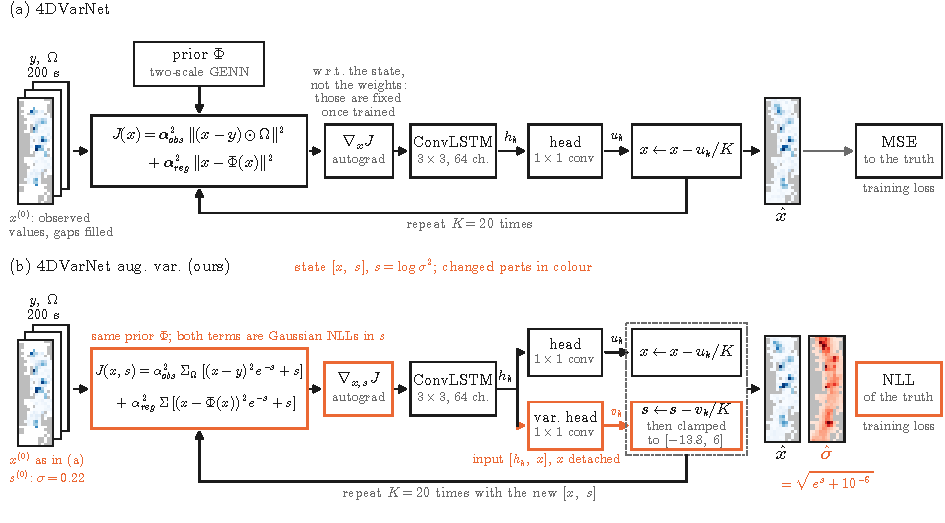
\includegraphics[width=\textwidth]{figures/varnet.pdf}
	\caption{(a) 4DVarNet. The variational cost $J$, with observations $y$, mask
	$\Omega$ and learned prior $\Phi$, guides a fixed sequence of learned
	updates: the gradient $\nabla_x J$ passes through a ConvLSTM, whose hidden
	state $h_k$ an output head turns into the update $u_k$ of the state; this is
	repeated 20 times, starting from the observations with gaps filled. The
	gradient is taken with respect to the state, not the weights, at inference as
	well as during training: the weights are fixed once the model is trained. (b) The
	augmented 4DVarNet proposed in this thesis has the same structure
	and iterates the state together with its log-variance $s$. The three changes
	are drawn in colour: both terms of the cost become Gaussian negative
	log-likelihoods in $s$, so that its gradient is taken with respect to $x$
	and $s$; a second output head, the variance head, updates $s$ from $h_k$ and
	the state detached from the graph, after which $s$ is clamped; and the model
	is trained with the negative log-likelihood of the truth, under the same
	$\hat{\sigma}^2 = e^{s} + 10^{-6}$ that it reports. The thumbnails show
	the density reconstructions of one test frame and the predicted
	$\hat{\sigma}$.}
	\label{fig:varnet}
\end{figure}

\subsubsection{4DVarNet with an augmented variance (ours)}
\label{sec:aughead}

The augmented 4DVarNet proposed in this thesis estimates the variance
inside the variational problem, rather than reading it off the network once the
state has been reconstructed (Figure~\ref{fig:varnet}b). The state that
the solver iterates is augmented to $[x, s]$, where $s = \log \sigma^2$ is
a per-cell, per-channel, per-frame log-variance.

This $\sigma^2$ is not the velocity variance $\nu$, and the two must be kept
apart. $\nu$ is the fourth channel of the state itself: how much the velocity
records inside a cell disagree, a property of the crowd that every
method has to reconstruct. $\sigma^2$ is the model's statement about its own
error, and the augmented state carries one value of it for each of the four
channels -- including a $\sigma^2$ for the estimate of $\nu$, that is, how
uncertain the model is about its reconstruction of the velocity variance.
Nothing in the plain 4DVarNet, or in the state itself, provides $\sigma^2$.

Both terms of the cost are replaced by Gaussian negative log-likelihoods in
$\sigma^2$:
\begin{equation}
	\begin{aligned}
	J(x, s) &= \alpha_{\mathrm{obs}}^2 \sum \Big( \big[ (x - y)^2 e^{-s} + s \big] \odot \Omega \Big) \\
	        &\quad + \alpha_{\mathrm{reg}}^2 \sum \Big[ \big(x - \Phi(x)\big)^2 e^{-s} + s \Big],
	\end{aligned}
	\label{eq:augcost}
\end{equation}
with squared per-channel coefficients as in Eq.~\eqref{eq:varcost}, both sums divided by the number of points per channel over the batch, time and grid, and the observation mask applied
inside the sum to both the squared residual and the log-variance penalty.
Ignoring the clamp, minimising $J$ with respect to $s$ alone gives $e^{s} = (x - \Phi(x))^2$ on unobserved cells: the variance
tracks the local disagreement between the state and the prior, and where a cell
is observed, also its disagreement with the observation. The solver thus refines
$\sigma^2$ over the $K$ iterations against the same cost as the state, rather
than producing it once from a hidden state.

\paragraph{Variance update.}
At each iteration, the gradients of $J$ with respect to $x$ and to $s$ are
concatenated, multiplied by the number of windows and normalised per window as in
the plain 4DVarNet, with $\|g_0\|_{\mathrm{rms}}$ taken over both, and passed to the
ConvLSTM, whose input therefore has $2 \times 800 = 1\,600$ channels instead of 800. The state is
updated as in Eq.~\eqref{eq:solver}, with a state-update head of the same architecture as in the plain 4DVarNet. The log-variance is updated by a second output head of the same kind
-- a $1 \times 1$ convolution -- which is the only module added to the network.
Its input is the LSTM hidden state concatenated with the current state $x$
($64 + 800 = 864$ channels), and its output $v_k$ the update of the
log-variance (800 channels):
$s^{(k+1)} = s^{(k)} - \frac{1}{K}\, v_k$. This variance head reads $h_k$
together with $x^{(k)}$ detached from the computational graph, that is,
treated as a constant when gradients are computed. The detach
blocks gradients from the variance head back to $x$ through this input feature;
the head still uses $x$ to predict the variance update. It does not decouple the two. The
state and the log-variance are updated from the same ConvLSTM, which is fed the
gradients of both; they appear together in the cost of
Eq.~\eqref{eq:augcost}, so each one's gradient depends on the other; and the
training loss of the next paragraph is a single likelihood in both. The variance
head is initialised to zero, so that before training its first forward pass
leaves $s$ at its initial value, $s^{(0)} = \log \mathrm{softplus}(-3)$, with $\mathrm{softplus}(a) = \log(1 + e^{a})$,
i.e., $\sigma \approx 0.22$.
After every update, and not only at the end, $s$ is clamped to $[-13.8, 6]$
($\sigma^2 \in [10^{-6}, e^{6}]$), which prevents the feedback between $s$,
$e^{-s}$ and the next gradient from diverging.

\paragraph{Training and output.}
The variance the model delivers is
\begin{equation}
	\hat{\sigma}^2 = e^{s^{(K)}} + 10^{-6},
	\label{eq:augvar}
\end{equation}
the $10^{-6}$ keeping it strictly positive and doubling the floor where the
clamp binds. The model is trained with the Gaussian negative log-likelihood of
the truth under $\mathcal{N}(x^{(K)}, \hat{\sigma}^2)$, averaged over all cells,
channels and frames, instead of the mean squared error. Its output is the state
$\hat{x} = x^{(K)}$ and the uncertainty $\hat{\sigma}$ of
Eq.~\eqref{eq:augvar}, within one invocation of the trained 20-step solver; the same
$\hat{\sigma}^2$ is the one the loss is computed with and the one reported in
Section~\ref{sec:res_unc}, so the floor is part of both. Apart from the augmented state, the
cost of Eq.~\eqref{eq:augcost}, the variance head and the loss, it uses the
same prior architecture, ConvLSTM type and hidden width, window, training
schedule and initialisation seed as the plain 4DVarNet. The models are trained separately with their own
weights; the augmented ConvLSTM input has twice as many channels.

\subsubsection{Localised ensemble Kalman filter}
\label{sec:enkf}

The EnKF is a localised filter with a learned forecast model and a running
correction of its bias (Figure~\ref{fig:enkf}). Its forecast model reads five
input frames, and its process noise is drawn from the forecast model's own
one-step errors. The filter represents the state distribution by an ensemble
of $N_e = 100$ members $x^{(i)}_t$ and runs
one forecast--analysis cycle per second.

\begin{figure}[htb]
	\centering
	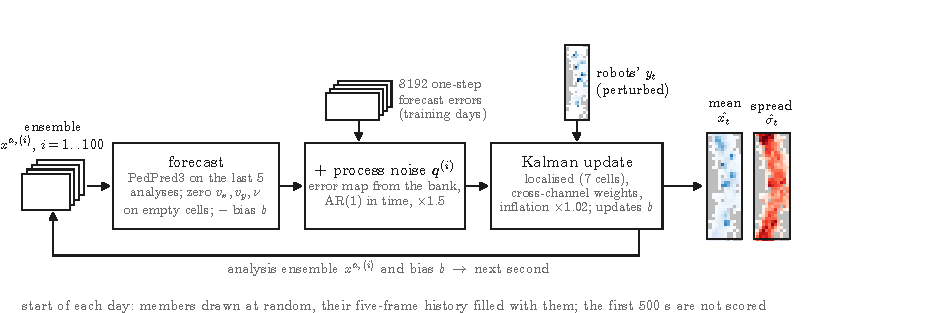
\includegraphics[width=\textwidth]{figures/enkf.pdf}
	\caption{The localised EnKF, one cycle per second. Each of the 100 members is
	advanced by the PedPred3 forecast model from its last five analyses; the
	velocity components and the velocity variance are set to zero on cells
	forecast as empty, and the running bias estimate $b$ is subtracted. Process
	noise drawn from a bank of real one-step forecast errors is added. In the
	Kalman step, $b$ is updated first, which takes effect in the next forecast;
	a localised update then assimilates the robots' perturbed observations and
	inflates the analysis anomalies. The ensemble mean and standard deviation are the estimate and
	its uncertainty, and the analysis ensemble is carried to the next second. At
	the start of each day the members are random, and the first 500\,s are not
	scored.}
	\label{fig:enkf}
\end{figure}

\paragraph{Forecast.}
The forecast model, PedPred3, is a convolutional recurrent network with an
encoder and a forecaster (Figure~\ref{fig:pedpred},
Table~\ref{tab:arch_pedpred}), following the encoding--forecasting structure that
\citeauthor{shi2017nowcasting} \cite{shi2015convlstm, shi2017nowcasting} use for
precipitation nowcasting. The encoder reads the input frames one by one:
three convolutions reduce each frame to $9 \times 3$ cells with 64 channels,
and a convolutional GRU combines it with its recurrent state, which is carried
from one frame to the next and so summarises the frames read so far. The
forecaster has a second convolutional GRU, which receives no input and starts
from the encoder's final state; transposed convolutions bring its output back
to $36 \times 12$ cells, and two convolutions produce the four output
channels. Each run of the forecaster produces one output frame. Both recurrent
units are convolutional GRUs \cite{cho2014gru} with 64 channels, which update
their state $h$ from an input $a$ as
\begin{equation}
	\begin{aligned}
	r &= \sigma\big(W_{ar} \ast a + b_{ar} + W_{hr} \ast h + b_{hr}\big), \\
	z &= \sigma\big(W_{az} \ast a + b_{az} + W_{hz} \ast h + b_{hz}\big), \\
	n &= \mathrm{LReLU}_{0.2}\big(W_{an} \ast a + b_{an} + r \odot (W_{hn} \ast h + b_{hn})\big), \\
	h &\leftarrow (1 - z) \odot n + z \odot h,
	\end{aligned}
	\label{eq:convgru}
\end{equation}
with the logistic sigmoid $\sigma$, the reset gate $r$, the update gate $z$, $3 \times 3$ convolutions $W_{a\cdot}$ on
the input and $5 \times 5$ convolutions $W_{h\cdot}$ on the state. Unlike the original
GRU, the candidate $n$ uses a leaky ReLU with slope 0.2 instead of a hyperbolic
tangent. The state of the encoder starts from zero; the GRU of the forecaster has
no input, so its terms in $W_{a\cdot}$ and $b_{a\cdot}$ are absent. The network outputs the
logarithm of the density, the mean velocity and the logarithm of the velocity
variance; the filter uses the corresponding forecast of the state. It is trained
on the ground-truth sequences of the training days to forecast the next five
frames from the previous five, with the weighted likelihood loss
\begin{equation}
	\mathcal{L}_{\mathrm{forecast}} = \frac{1}{N} \sum_j
	\left\{
	\hat{\rho}_j - \rho_j \log \hat{\rho}_j
	+ \rho_j \left[
	\frac{\|\hat{\boldsymbol{v}}_j - \boldsymbol{v}_j\|_2^2}{2\hat{\nu}_j}
	+ \frac{\nu_j}{\hat{\nu}_j} + \log \hat{\nu}_j
	\right]
	\right\},
	\label{eq:pedpred_loss}
\end{equation}
where $j$ indexes the $N$ cell values over the batch and forecast frames,
$\boldsymbol{v}=(v_x,v_y)$, unhatted quantities are the ground-truth targets and
hatted quantities the decoded network outputs before any filter
post-processing; $\hat{\rho}$ and $\hat{\nu}$ are positive through their
exponential parametrisation. The first two terms form a Poisson-type likelihood
of the density; the velocity terms are weighted by the true density and vanish
where it is zero. Here $\hat{\nu}$ is the forecast of the crowd's velocity
dispersion, not a predictive error variance: the four state outputs serve both
the forecast and this loss, and there is no separate error-variance output.
The checkpoint is selected on the validation days by its one-step forecast
loss (Section~\ref{sec:impl}).
The filter's predictive uncertainty comes from ensemble spread.

In the filter, each member is advanced one second from its own last five
analysed states. The forecast that the filter propagates is not the raw network
output: the network's velocity and velocity-variance channels are never trained
on empty cells, because the training loss weights them by the true density, so
they drift there. The two velocity components and the velocity variance are
therefore set to zero wherever the forecast density is below 0.01, and the
result is clipped to the bounds of Section~\ref{sec:eval}. The threshold was
chosen during the Sunday-only development, on its validation days, where 0.01
and 0.02 give the same error and 0.01
zeroes fewer occupied cells; without the zeroing the velocity-variance RMSE on
the validation days is 0.51--0.73 instead of 0.11. The full forecast chain is
thus: the network's output, decoded from the logarithm of the density and of the
velocity variance, the zeroing on empty cells, the clipping, the bias
correction, and the process noise.

The bias correction subtracts a state $b_t$ from each forecast,
$x^{f,(i)}_t = f\big(x^{a,(i)}_{t-5:t-1}\big) - b_t$, where $f$ is the zeroed and
clipped forecast described above. At each analysis,
observed components are updated by
$b \leftarrow 0.95\, b + 0.05\,(\bar{x}^f-y_t)$, where $\bar{x}^f$ is the
already corrected forecast ensemble mean. This is a heuristic feedback
correction rather than a direct estimate of the raw forecast bias.

\begin{figure}[htb]
	\centering
	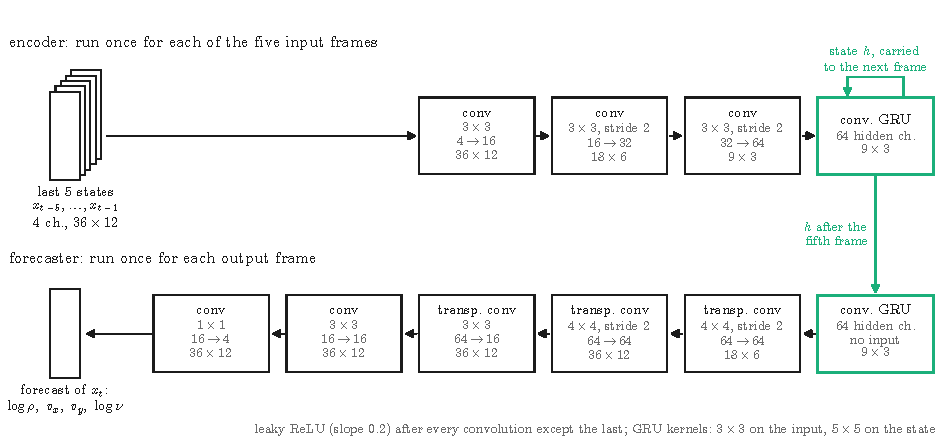
\includegraphics[width=\textwidth]{figures/pedpred.pdf}
	\caption{The PedPred3 forecast model of the EnKF. The encoder (top) is run
	once for each of the five input frames; its convolutional GRU carries a
	recurrent state $h$ from frame to frame. The forecaster (bottom) starts from
	the state after the fifth frame and is run once for each output frame; the
	filter uses the first output frame as the forecast of the next second. Each
	box gives the kernel size, the number of channels and the size of the output
	grid.}
	\label{fig:pedpred}
\end{figure}

\begin{table}[htb]
	\centering
	\caption{Layers of the PedPred3 forecast model of the EnKF. Every convolution
	except the last is followed by a leaky ReLU with slope 0.2. The convolutional
	GRUs have 64 hidden channels, with a $3 \times 3$ kernel on the input and a
	$5 \times 5$ kernel on the hidden state.}
	\label{tab:arch_pedpred}
	\small
	\begin{tabular}{llll}
		\hline
		Part & Operation & Channels & Output size \\
		\hline
		Encoder    & convolution $3 \times 3$ & $4 \to 16$ & $36 \times 12$ \\
		           & convolution $3 \times 3$, stride 2 & $16 \to 32$ & $18 \times 6$ \\
		           & convolution $3 \times 3$, stride 2 & $32 \to 64$ & $9 \times 3$ \\
		           & convolutional GRU & 64 & $9 \times 3$ \\
		Forecaster & convolutional GRU & 64 & $9 \times 3$ \\
		           & transposed convolution $4 \times 4$, stride 2 & $64 \to 64$ & $18 \times 6$ \\
		           & transposed convolution $4 \times 4$, stride 2 & $64 \to 64$ & $36 \times 12$ \\
		           & transposed convolution $3 \times 3$ & $64 \to 16$ & $36 \times 12$ \\
		           & convolution $3 \times 3$ & $16 \to 16$ & $36 \times 12$ \\
		           & convolution $1 \times 1$ & $16 \to 4$ & $36 \times 12$ \\
		\hline
	\end{tabular}
\end{table}

\paragraph{Structured process noise.}
In place of independent Gaussian process noise, each member receives a whole
field $q^{(i)}_t$ drawn from a bank of 8\,192 one-step forecast errors of the
forecast model, $x_{t+1} - f(x_{t-4:t})$, computed on the ground truth of the
training days, with their mean removed; each drawn field keeps the spatial and
cross-channel correlations of a real forecast error, and its size is the size
of the model's actual one-step error, not a prescribed per-channel standard
deviation. For density, the error is taken and
added in $\log(1+\rho)$ space, and the resulting shift of the ensemble mean is
removed. The noise is correlated in time through a first-order autoregressive, AR(1), process with
coefficient 0.5 and scaled by 1.5; the draws are centred over the ensemble.
The 8\,192 errors are drawn at random, without replacement, from the scored
frames of the 63 training days (Section~\ref{sec:gridding}), 130 or 131 per day
so that no day dominates, and the forecast in them is the zeroed and clipped
forecast that the filter propagates. In the filter, each member draws one field
from the bank, uniformly and with replacement, at every second.

\paragraph{Analysis.}
The analysis is a stochastic EnKF update with perturbed observations
\cite{burgers1998enkf, roth2017enkf}: each member assimilates its own noisy copy of the
observations of all observed cells and channels. Let $\mathcal{H}_t$ select the
$4 N_s$ observed components of the state, let $R$ be the observation error
covariance, formed by repeating the four-channel diagonal
$\mathrm{diag}(\sigma^2_{\mathrm{obs}})$ over the observed cells, and let
$A = \big[\, x^{f,(1)} - \bar{x}^f, \dots, x^{f,(N_e)} - \bar{x}^f \,\big]$ be
the forecast anomalies and $B = \mathcal{H}_t A$ their observed part. The gain and its
localised form are
\begin{equation}
	\begin{aligned}
	G &= \frac{A B^{\top}}{N_e - 1} \left( \frac{B B^{\top}}{N_e - 1} + R + 10^{-3} I \right)^{-1}, \\
	\tilde{G}_{(c, j), (c', l)} &= G_{(c, j), (c', l)}\; \varrho(d_{jl})\; \Lambda_{c c'},
	\qquad
	\varrho(d) = \begin{cases} \exp\!\big(-d^2 / 2 r^2\big), & d \le r, \\ 0, & d > r, \end{cases}
	\end{aligned}
	\label{eq:enkf_gain}
\end{equation}
where $(c, j)$ is channel $c$ of cell $j$ and $(c', l)$ channel $c'$ of the
observed cell $l$, $d_{jl}$ is the Euclidean distance between the centres of
the two cells, measured in cells, $r = 7$, and $\Lambda$ is a fixed cross-channel matrix (1
between a channel and itself, 0.5 among density and the two velocity
components, 0.1 between the velocity variance and the others). The
localisation therefore multiplies the gain, not the covariance. The gain is
evaluated in the $N_e$-dimensional space of the ensemble, through the
equivalent form $G = A \big( (N_e - 1) I + B^{\top} D^{-1} B \big)^{-1}
B^{\top} D^{-1}$ with $D = R + 10^{-3} I$, so only an $N_e \times N_e$ system
is solved. Every member is then updated with its own perturbed observation, and
the analysis anomalies are inflated,
\begin{equation}
	\begin{aligned}
	x^{a,(i)} &= x^{f,(i)} + \tilde{G} \big( y_t + \varepsilon^{(i)} - \mathcal{H}_t x^{f,(i)} \big),
	\qquad \varepsilon^{(i)} \sim \mathcal{N}(0, R), \\
	x^{a,(i)} &\leftarrow \bar{x}^a + 1.02 \big( x^{a,(i)} - \bar{x}^a \big),
	\end{aligned}
	\label{eq:enkf_update}
\end{equation}
after which every member is clipped to the fixed bounds of the state. The
$10^{-3} I$ in the gain is a numerical regularisation. Its largest relative
effect is on velocity variance, whose standard deviation in the gain becomes
about 0.032 instead of 0.0064. Members are perturbed with $R$ itself, so the
gain and observation perturbations use different effective covariances.

\paragraph{Output and configuration.}
The estimate is the ensemble mean, $\hat{x}_t = \bar{x}^a_t$, and the
uncertainty the ensemble standard deviation, $\hat{\sigma}_t$, both computed over
the 100 members with divisor $N_e$. At the start of each day, every member is
drawn independently in every cell from a zero-mean Gaussian with standard
deviations $(0.028,\ 0.31,\ 0.12,\ 0.42)$ for $(\rho, v_x, v_y, \nu)$ and
clipped to the fixed bounds, and the five-frame history of each member is
filled with this initial state. The filter starts without knowledge of
the crowd and needs some time to converge; the first 500\,s of each day are therefore
discarded as warm-up. The process-noise settings were chosen during the Sunday-only
development, on its validation days. The noise scale and its temporal
correlation come from an earlier sweep and were kept when PedPred3 became the
forecast model. With the PedPred3 of that development, the bank fields were then
kept at this measured size instead of being rescaled to prescribed per-channel
standard deviations, and the variant without additional per-channel
multipliers of the noise was selected among the process-noise candidates (Section~\ref{sec:impl}). The
localisation radius, the inflation factor, the bias update and the
cross-channel matrix were not part of the validation sweeps.

\paragraph{One cycle, step by step.}
The order of the operations within one second $t$ is as follows
(Figure~\ref{fig:enkf}); it is the order of the implementation, and every step
uses only the observations up to $t$.
\begin{enumerate}
	\item \emph{Forecast.} Each member $i$ is advanced by PedPred3 from its last
	five analyses $x^{a,(i)}_{t-5:t-1}$. The velocity components and the velocity
	variance are set to zero where the forecast density is below 0.01 and the
	result is clipped to the fixed bounds; the current bias estimate $b_t$
	is then subtracted and the result clipped again.
	\item \emph{Process noise.} One field is drawn from the bank of one-step
	forecast errors for each member and passed through the AR(1) recursion
	$q^{(i)}_t = 0.5\, q^{(i)}_{t-1} + \sqrt{1 - 0.5^2}\; \tilde{q}^{(i)}_t$, where
	$\tilde{q}^{(i)}_t$ is the new draw and $q^{(i)}$ starts from zero each day; the
	factor $\sqrt{1 - 0.5^2}$ makes the stationary variance of $q$ equal to that
	of a single draw, which $q$ approaches within the first few steps after its
	zero start. The fields
	are multiplied by 1.5 and centred over the ensemble, and added to the
	forecasts: to $\log(1+\rho)$ for the density, with the resulting shift of the
	ensemble mean removed, and directly for the other channels. The members are
	clipped again.
	\item \emph{Bias update.} On the observed components, the bias estimate is
	moved towards the difference between the forecast ensemble mean and the
	observation, $b \leftarrow 0.95\, b + 0.05\,(\bar{x}^f - y_t)$; it takes
	effect from the next forecast.
	\item \emph{Analysis.} The localised gain of Eq.~\eqref{eq:enkf_gain} is
	computed from the forecast anomalies, and each member is updated with its own
	perturbed copy of the observation and inflated as in
	Eq.~\eqref{eq:enkf_update}; the members are then clipped. In a second without
	any observed cell, the analysis equals the forecast. On the test days, the
	linear system of the gain was solved in every cycle; no analysis was skipped.
	\item \emph{Output.} The ensemble mean and standard deviation of the
	analysis are the estimate and the uncertainty for second $t$, and each
	member's analysis is appended to its five-frame history.
\end{enumerate}


%% ------------------------------------------------------------------
\FloatBarrier
\subsection{Evaluation protocol}
\label{sec:eval}

All methods are evaluated on the 15 test days, with the same
observations, along the three axes of Section~\ref{sec:intro}: reconstruction
accuracy, uncertainty quality and computational cost.

\paragraph{Scored cells.}
Accuracy is scored on all walkable cells $\mathcal{W}$, observed ones included,
and separately on the blind cells $\mathcal{B}_t$ of Eq.~\eqref{eq:blind}:
the walkable cells that no robot observes at that second, about 44\% of the
walkable cells. The uncertainty is scored on both sets of cells, like the
accuracy; the error breakdown uses the blind cells. Empty cells are included: correctly reconstructing that a cell
is empty is part of the task.

\paragraph{Reconstruction accuracy.}
Accuracy is measured by the root-mean-square error, pooled over all scored
cells of all test frames,
\begin{equation}
	\mathrm{RMSE} = \sqrt{ \frac{1}{N} \sum_{t} \sum_{j \in \mathcal{S}_t} \sum_{c=1}^{C}
	\big( \hat{x}_{t,c,j} - x_{t,c,j} \big)^2 },
	\label{eq:rmse}
\end{equation}
where $\mathcal{S}_t$ is the set of scored cells, $\mathcal{W}$ or $\mathcal{B}_t$,
$N = C \sum_t |\mathcal{S}_t|$ is the number of scored values, with $C = 4$ for the pooled score, reported next to the RMSE of each channel
($C = 1$) in its own physical unit. Pooled scores combine channel errors with
equal numerical weight in those stated units and have no single physical unit.
Every point prediction is clipped to the
fixed bounds of the state (density in $[0, 5]$, velocity in $[-5, 5]$,
velocity variance in $[0, 2]$) before scoring, as the EnKF does internally.
All frames of each day are scored except the first and the last, for which
DINCAE lacks a neighbouring frame. There are two exceptions. For the EnKF, the
scored frames run from the end of its 500-frame warm-up, which excludes about the first
1.3\% of each day, to the last frame of the day. For the two 4DVarNet models, the frames after the last complete
200-frame window of a day (fewer than 200 frames, up to about 0.5\% of a day) are
not reconstructed and not scored. For every method, the blocks affected by
recording gaps (Section~\ref{sec:gridding}) are also excluded, 1.5\% of the
test frames.

\paragraph{Uncertainty quality.}
The three probabilistic methods are scored on one common protocol: the frames
after the EnKF warm-up that also lie within complete 4DVarNet windows and
outside the blocks affected by recording gaps, which are the frames on which
all methods can be compared
(Section~\ref{sec:res_breakdown}), and the same cells, all walkable cells and,
separately, the blind cells. Distributions are scored in physical units
without additional clipping; the EnKF retains its internal member clipping.
The primary
score is the CRPS
\cite{gneiting2007scoring}, defined in Eq.~\eqref{eq:bg_crps}. For the Gaussian
outputs of the augmented 4DVarNet and DINCAE, it is calculated
from the corresponding Gaussian distribution. The EnKF outputs an ensemble rather than a
parametric distribution, so its CRPS is calculated from its $N_e$ members. For a
distribution $F$ with a finite first moment, Eq.~\eqref{eq:bg_crps} can be
written as $\mathrm{CRPS}(F, x) = \mathbb{E}_F |X - x| - \tfrac{1}{2}
\mathbb{E}_{F,F} |X - X'|$ with $X, X'$ independent and distributed as $F$
\cite{gneiting2007scoring}; taking $F$ to be the empirical distribution of the
members gives
\begin{equation}
	\mathrm{CRPS} = \frac{1}{N_e} \sum_i \big| x^{a,(i)} - x \big|
	- \frac{1}{2 N_e^2} \sum_i \sum_j \big| x^{a,(i)} - x^{a,(j)} \big| .
	\label{eq:crps_ens}
\end{equation}
This makes no assumption about the shape of the ensemble distribution, so it
also charges the filter for the skewness and the clipping at zero that a
mean-and-spread summary hides.
The CRPS is averaged over all scored cells, per channel and
pooled over the four channels. As a second, simpler check of the overall size
of $\hat{\sigma}$, the ratio of the root-mean-square predicted standard
deviation to the RMSE \cite{dirkson2025spread} is reported,
\begin{equation}
	\frac{\mathrm{spread}}{\mathrm{RMSE}} =
	\sqrt{ \frac{\sum \hat{\sigma}^2}{\sum (\hat{x} - x)^2} },
	\label{eq:spread}
\end{equation}
with both sums over the same scored cells. A ratio of one means that the
RMS predictive spread equals the point-estimate RMSE; below one the
predictions are underdispersed relative to the pooled RMSE, above one
overdispersed. The ratio compares two separately averaged second moments, so it
cannot tell whether $\hat{\sigma}$ is large in the right cells, and a ratio of one is a
necessary but not a sufficient second-moment condition for calibration when
$\hat{x}$ is the predictive mean \cite{dirkson2025spread}.

As a direct check of the stated intervals, the coverage of the central 50\%
and 90\% prediction intervals is reported on the same frames and cells: the
fraction of true values inside the interval, with the nominal values 0.50 and
0.90. For the Gaussian outputs of the augmented 4DVarNet and DINCAE the
intervals are $\hat{x} \pm 0.674\,\hat{\sigma}$ and
$\hat{x} \pm 1.645\,\hat{\sigma}$; for the EnKF they are the empirical 0.25--0.75
and 0.05--0.95 quantiles of the members, with linear interpolation and the end
points included. The coverage is reported for the density, for the two
velocity components pooled and for the velocity variance.

\paragraph{Variability over test days.}
To show how much the uncertainty scores depend on which days happened to be the
test days, 95\% intervals of the pooled scores are computed with a bootstrap over days \cite{efron1979bootstrap}:
the 15 test days are resampled with replacement 10\,000 times.
Each resample combines the saved daily sums and counts and recomputes the
pooled score, retaining the weighting by scored values.

\paragraph{Computational cost.}
Compute time is measured on one NVIDIA Tesla V100-SXM2-16GB using prepared
inputs from a 600-frame test sequence and the context required by each method.
The reported value is the median per reconstructed frame over three repetitions.
These are small tensors on a $36 \times 12$ grid, so the measurement is
sensitive to the host as well as to the graphics processing unit (GPU). The times and ratios quoted below
refer to this benchmark, in which all final models were timed on the same GPU
and the same frames.
The two 4DVarNet models reconstruct a 200-frame window at once, so their time per
frame is the time per window divided by 200. The EnKF time includes prediction of all 100
members, the analysis update, and transfer of the posterior mean and spread
to the central processing unit (CPU). Input preparation, final scoring and file saving are excluded.

%% ------------------------------------------------------------------
\subsection{Implementation details}
\label{sec:impl}

All models are implemented in PyTorch and trained on single NVIDIA GPUs of the
Aalto Triton cluster with the Adam optimiser \cite{kingma2015adam}; Senseiver,
DINCAE and the two 4DVarNet models use mixed-precision arithmetic, which
carries out part of the computation in 16-bit floating point to save memory
and time. Table~\ref{tab:training}
lists the training configuration of each learned model. To reduce the
redundancy between adjacent seconds, Senseiver and DINCAE use every fourth
frame as a training target; their observation context retains its one-second
sampling. Thus Senseiver\nobreakdash-G reads consecutive past observations and DINCAE
uses the adjacent seconds. The two 4DVarNet models train on non-overlapping
200-frame windows within each day, discard incomplete tails, and shuffle the
windows each epoch. PedPred3 uses overlapping sequences of five historical
and five future frames, with a one-second stride. No training sample crosses
a day boundary. An epoch is one pass over the training samples.

The order of the samples is shuffled in every epoch. Senseiver, 4DVarNet and
PedPred3 shuffle all their training samples together, and Senseiver leaves out
the last, incomplete batch of each epoch; DINCAE, whose inputs are encoded day
by day, shuffles the order of the days and then reads four days at a time,
shuffling the frames within those four days.
The random seeds are 123 for both Senseiver models (weight initialisation; the
sample order of epoch $e$ is drawn from a generator seeded with $(123, e)$), 3
for the weight initialisation of the two 4DVarNet models, and 0 for PedPred3.
DINCAE seeds its sample order with the epoch number but not its weight
initialisation, which therefore cannot be repeated exactly. During training,
each run also records a monitoring score after every epoch, which is not used
for the final selection: the blind-cell MSE on 40 batches of every 20th frame
of three validation days for Senseiver, the loss on every 16th frame of the validation
days for DINCAE, the blind-cell MSE on the first 1\,024 training windows for
4DVarNet (its ``training-monitor best'' snapshot), and the validation forecast
loss for PedPred3, which also drives its learning-rate schedule. The software is
PyTorch 2.10, and the weights not stated otherwise use the default
initialisation of PyTorch.

The EnKF is not reproducible bit for bit. Two runs with the same seeds on the
same GPU differ by about $3 \cdot 10^{-7}$ in the first frame, the size of a
single-precision rounding difference, and visibly in individual cells within
about 50 frames. The coverage of the EnKF in Table~\ref{tab:coverage} comes from
a rerun with the same configuration, because the reported run did not store its
members.

For 4DVarNet, seed 3 was
chosen from five earlier fixed-route runs by validation error; the reported
final model was then trained once with that seed and day-specific routes, and
the augmented 4DVarNet with the same seed and routes. Each other reported
learned model is represented by one final run. No result is an ensemble of networks.
The final checkpoints of all five observation-conditioned reconstruction models
are selected by the lowest pooled MSE on all walkable cells, observed and blind,
over all scored frames (Section~\ref{sec:gridding}) and four channels of the 14
validation days, with point
estimates clipped to the bounds of Section~\ref{sec:eval}, irrespective of the
training loss. The candidates are every saved epoch of Senseiver\nobreakdash-A (0--99),
Senseiver\nobreakdash-G (0--59) and DINCAE (0--149); and, for the two 4DVarNet models, the
snapshots at the final depth $K = 20$ (epochs 80, 90 and 100 for both) together
with the training-monitor best and last snapshots. Of a maximum budget of 150
epochs, the 4DVarNet run met its stopping rule at the epoch-100 check, when its
best $K = 20$ snapshot under the same criterion (epoch 80) was 20 epochs old,
and ended after epoch 104. The augmented
4DVarNet run was stopped after epoch 104 to bound the training time, although
its validation error was still decreasing slowly (pooled RMSE 0.2223, 0.2212
and 0.2205 at epochs 80, 90 and 100, and 0.2200 at the selected epoch 104).
The EnKF configuration of Table~\ref{tab:selection} is kept from the
Sunday-only development without being scored again. PedPred3 is selected by
the forecast loss of Eq.~\eqref{eq:pedpred_loss} on the validation days for
the forecast the EnKF uses: one step ahead from the true past five frames,
clipped to the EnKF's bounds (see below).

Senseiver and DINCAE keep their learning rates constant. DINCAE uses an
$L_2$ weight penalty of $10^{-4}$ and clips every gradient component to
$[-5, 5]$; 4DVarNet and its augmented variant clip the gradient norm at 1.
PedPred3 uses Adam with AMSGrad and a plateau scheduler that halves the
learning rate once the validation loss of its five-step forecast has not
improved for more than 10 epochs (patience 10), and restarts this count
immediately after a reduction (no cooldown); only a strictly lower loss counts
as improvement.
In the first training run this five-step validation loss became unstable from
epoch 18 on (non-finite at epochs 18, 19 and 21): fed back over five steps, the forecast diverges on frames of
a recording gap. The run was restarted from the epoch-14 weights with a fresh
optimiser, an initial learning rate of $5 \cdot 10^{-4}$ and gradient clipping
at 1; its five-step validation loss remained unstable, and the restart was
stopped after epoch 23. The 47 checkpoints of both runs were therefore compared
by the one-step validation loss described above, which selects epoch 23 of the
restart, trained at $1.25 \cdot 10^{-4}$.

\paragraph{Selection of the designs.}
The design choices listed in Table~\ref{tab:selection} were made during the
Sunday-only development, on its seven validation Sundays, by comparing
candidate designs, one seed each (the Senseiver
candidates for 40 instead of 60 epochs). The decision rules were committed
before the new candidate runs were trained; as the protocol specifies, the
comparison also reused runs trained earlier for the Senseiver\nobreakdash-A and
Senseiver\nobreakdash-G ($L = 16$) candidates.
The observation-conditioned candidates used one route realisation
replayed across days. After fixing the designs, all observation-conditioned
models were retrained with per-day routes, and PedPred3 on the ground truth,
on the 63 training days of the present split, and their final checkpoints
were selected on its 14 validation days. Each candidate is scored by its
pooled RMSE on the blind walkable cells of every validation frame at its best
validation epoch; the EnKF configurations are compared by the
Gaussian-summary CRPS of their ensemble mean and spread, as fixed in the
validation protocol, among the candidates whose RMSE is at most 5\% above that
of the error-bank noise without per-channel factors. For Senseiver\nobreakdash-G,
the grid-aligned latent array is compared with the abstract latent array of
Senseiver\nobreakdash-A, and the window length among $L \in \{1, 4, 8, 16\}$, a window
being admissible only if no channel is more than 5\% less accurate than without
a window. The
reported test evaluation was run after all final models had been fixed.
The prior of the two 4DVarNet models was not selected in this comparison: its
width of 96 channels was taken over from a pilot implementation, which had a
different channel--time ordering in the coarse branch and whose scores are
therefore not reported, and its temporal kernel $k_t = 3$ was set directly.
Both final models use the corrected ordering described in
Section~\ref{sec:varnet}.

\begin{table}[htb]
	\centering
	\caption{Training configuration of the learned models. Learning rates are
	initial values; the schedules are stated in the text. Batch counts target
	frames for Senseiver and DINCAE, complete windows for 4DVarNet, and
	history--future sequences for PedPred3. Epochs give the zero-based index of
	the selected epoch and the number of epochs trained. The two 4DVarNet models
	and PedPred3 had a budget of 150 epochs and were stopped earlier, as described
	in the text; PedPred3 counts the restart, which followed 23 epochs of a first
	run. Every model was selected on all 14 validation days. Parameters count the
	trained weights.}
	\label{tab:training}
	\small
	\setlength{\tabcolsep}{3pt}
	\begin{tabular}{llllll}
		\hline
		Model & Loss & Batch & Initial LR & Epochs & Parameters \\
		\hline
		Senseiver\nobreakdash-A          & sum of squared errors & 64 & $10^{-3}$ & 97 / 100 & 65\,892 \\
		Senseiver\nobreakdash-G (ours)   & sum of squared errors & 64 & $10^{-3}$ & 57 / 60 & 56\,676 \\
		DINCAE               & Gaussian NLL          & 64 & $10^{-3}$ & 6 / 150 & 319\,696 \\
		4DVarNet             & MSE                   & 32 & $10^{-3}$ & 80 / 105 & 2\,082\,518 \\
		4DVarNet aug.\ var.\ (ours) & Gaussian NLL          & 32 & $10^{-3}$ & 104 / 105 & 4\,616\,918 \\
		PedPred3 (EnKF)      & weighted likelihood          & 64 & $5 \cdot 10^{-4}$ & 23 / 24 & 892\,116 \\
		\hline
	\end{tabular}
\end{table}

\begin{table}[htb]
	\centering
	\caption{Design choices made on the seven validation Sundays of the
	Sunday-only development, one seed per candidate (Senseiver candidates trained
	for 40 epochs). Scores: pooled RMSE on the blind walkable cells; for the EnKF,
	the CRPS of the Gaussian summary of the ensemble, followed by its RMSE.
	Per-channel factors are additional per-channel multipliers of the process
	noise. The selected design is in bold.}
	\label{tab:selection}
	\small
	\setlength{\tabcolsep}{4pt}
	\begin{tabular}{L{0.27\textwidth}L{0.67\textwidth}}
		\hline
		Choice & Candidates (validation score) \\
		\hline
		Senseiver\nobreakdash-G latent array & abstract, 64 latents (0.213); \textbf{grid, one token per cell (0.210)} \\
		Senseiver\nobreakdash-G window $L$ & 1\,s (0.210); 4\,s (0.197); 8\,s (0.192); \textbf{16\,s (0.189)} \\
		EnKF process noise & independent Gaussian (0.151, 0.302); error bank with per-channel factors on the blind cells (0.112, 0.254); error bank with per-channel factors on all cells (0.112, 0.252); \textbf{error bank without per-channel factors (0.104, 0.245)} \\
		\hline
	\end{tabular}
\end{table}

All observation-conditioned learned models (Senseiver\nobreakdash-A, Senseiver\nobreakdash-G,
DINCAE, 4DVarNet and the augmented 4DVarNet) were trained with
robot routes seeded separately for each day, as described in
Section~\ref{sec:obs}. The validation and test days also have their own
routes, which no model has seen during training, and all methods are evaluated
on identical test observations. PedPred3 is trained on the ground truth alone
and does not depend on the routes.

\clearpage

\section{Results and discussion}
\label{sec:results}

This section presents the results of the evaluation described in
Section~\ref{sec:eval}: the reconstruction accuracy of the six methods
(Section~\ref{sec:res_acc}), an example of their reconstructions
(Section~\ref{sec:res_example}), a breakdown of where their errors occur
(Section~\ref{sec:res_breakdown}), the quality of the uncertainty predicted by the
three probabilistic methods (Section~\ref{sec:res_unc}), and the computational
cost of all six (Section~\ref{sec:res_cost}). Section~\ref{sec:discussion}
answers the research questions and discusses the limitations of the study. All
numbers are computed over the 15 test days. Accuracy is reported on all
walkable cells and on the blind cells, and so is the uncertainty; the example
and the error breakdown use the blind cells.

The methods use different temporal information (Table~\ref{tab:methods}).
DINCAE uses the next second and the two 4DVarNet models the whole 200-second
window, both including observations after the reconstructed frame, whereas
Senseiver\nobreakdash-A, Senseiver\nobreakdash-G and the EnKF use only current and past observations.
This difference matters when their accuracy is compared and for their use
online.

%% ------------------------------------------------------------------
\subsection{Reconstruction accuracy}
\label{sec:res_acc}

Table~\ref{tab:accuracy} and Figure~\ref{fig:accuracy} give the RMSE of every
method, pooled over the four channels and for each channel, on all walkable
cells, observed ones included (left half of the table, Figure~\ref{fig:accuracy}a),
and on the blind cells alone (right half, Figure~\ref{fig:accuracy}b).

\begin{table}[htb]
	\centering
	\caption{Reconstruction RMSE on the 15 test days, pooled over the four
	channels (``All'') and per channel, on all walkable cells, observed and
	blind (left), and on the blind cells (right). Physical units apply to the
	per-channel columns; pooled values have no single physical unit. Lower is
	better; the lowest value of each column is in bold.}
	\label{tab:accuracy}
	\small
	\setlength{\tabcolsep}{4pt}
	\resizebox{\textwidth}{!}{%
	\begin{tabular}{lccccc|ccccc}
		\hline
		& \multicolumn{5}{c|}{All walkable cells} & \multicolumn{5}{c}{Blind cells} \\
		\cline{2-11}
		Method & All & $\rho$ & $v_x$ & $v_y$ & $\nu$ & All & $\rho$ & $v_x$ & $v_y$ & $\nu$ \\
		\hline
		Senseiver\nobreakdash-A        & 0.144 & 0.093 & 0.242 & 0.102 & 0.068 & 0.206 & 0.133 & 0.347 & 0.147 & 0.094 \\
		Senseiver\nobreakdash-G (ours) & \textbf{0.125} & \textbf{0.077} & \textbf{0.209} & \textbf{0.094} & \textbf{0.064} & \textbf{0.182} & \textbf{0.113} & \textbf{0.303} & \textbf{0.137} & \textbf{0.091} \\
		DINCAE             & 0.176 & 0.117 & 0.296 & 0.125 & 0.083 & 0.214 & 0.136 & 0.362 & 0.157 & 0.098 \\
		4DVarNet           & 0.181 & 0.108 & 0.307 & 0.136 & 0.085 & 0.212 & 0.152 & 0.335 & 0.172 & 0.124 \\
		4DVarNet aug.\ var.\ (ours) & 0.226 & 0.114 & 0.407 & 0.138 & 0.085 & 0.276 & 0.162 & 0.481 & 0.178 & 0.125 \\
		EnKF               & 0.199 & 0.112 & 0.334 & 0.139 & 0.126 & 0.235 & 0.131 & 0.382 & 0.170 & 0.171 \\
		\hline
	\end{tabular}}
\end{table}

\begin{figure}[htb]
	\centering
	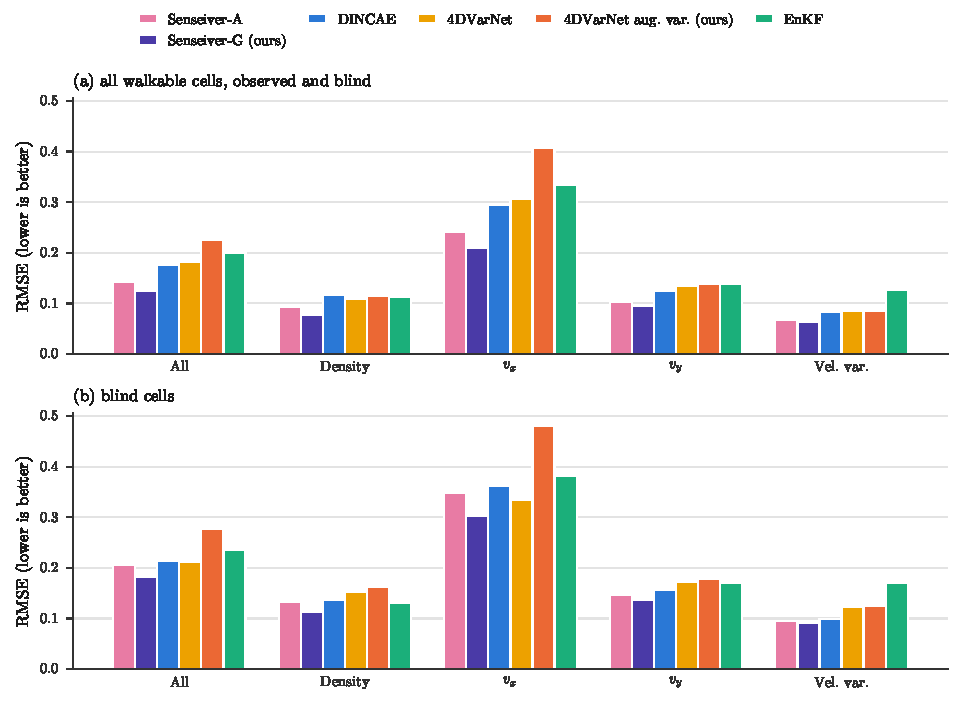
\includegraphics[width=\textwidth]{figures/accuracy.pdf}
	\caption{Reconstruction RMSE on the 15 test days, pooled over the four
	channels (left group) and per channel: (a) on all walkable cells, observed
	and blind, with the values of the left half of Table~\ref{tab:accuracy};
	(b) on the blind cells, with the values of its right half. Both panels share one
	axis. Lower is better.}
	\label{fig:accuracy}
\end{figure}

\paragraph{Senseiver\nobreakdash-G is the most accurate method.}
Senseiver\nobreakdash-G has the lowest error of all six methods, on all walkable cells
and on the blind cells, pooled and on every channel. On all walkable cells, its
pooled RMSE, 0.125, is 12.7\% lower than that of Senseiver\nobreakdash-A, 28.7\% lower than
DINCAE's and 31.0\% lower than that of 4DVarNet; on the blind cells, its pooled
RMSE, 0.182, is 11.7\%, 15.2\% and 14.5\% lower than theirs. The advantage is
largest on the density, where its RMSE is 17\% (all walkable cells) and 13\%
(blind cells) below the next best value. This is achieved by a causal model, which uses only the
current and past observations, against DINCAE and the two 4DVarNet models, which also see
observations after the reconstructed frame. The two changes of Senseiver\nobreakdash-G, the
grid-aligned latent array and the 16-second window, give the lowest error
in the reported comparison.

\paragraph{The augmented 4DVarNet.}
The augmented 4DVarNet is the least accurate of the six methods. Its pooled
RMSE is 24.9\% higher than that of the plain 4DVarNet on all walkable cells (0.226
against 0.181) and 30.0\% higher on the blind cells (0.276 against 0.212). The
difference lies mostly in $v_x$, whose blind-cell RMSE is 43.7\% higher (0.481
against 0.335); on the density, $v_y$ and the velocity variance it is 6.3\%,
3.3\% and 0.7\% higher.

\paragraph{All walkable cells and blind cells.}
Every method has a lower error on all walkable cells than on the blind cells
alone. On all walkable cells the pooled ranking is Senseiver\nobreakdash-G, Senseiver\nobreakdash-A,
DINCAE, 4DVarNet, the EnKF and the augmented 4DVarNet; on the blind cells
4DVarNet (0.212) moves just ahead of DINCAE (0.214), and the rest of the order
is the same. On all walkable cells, Senseiver\nobreakdash-A has the second lowest error,
pooled and on every channel. The density channel changes order the most: on all
walkable cells 4DVarNet (0.108) is more accurate than the EnKF (0.112) and
DINCAE (0.117), whereas on the blind cells the EnKF (0.131) and DINCAE (0.136)
are more accurate than 4DVarNet (0.152).

\paragraph{The EnKF is the second most accurate method on blind-cell density.}
On the blind cells, the EnKF reaches a density RMSE of 0.131, below those of
Senseiver\nobreakdash-A (0.133), DINCAE (0.136) and both 4DVarNet models; only Senseiver\nobreakdash-G
(0.113) is more accurate on this channel. This order is not an effect of the
EnKF's shorter scoring window (Section~\ref{sec:eval}): on the common frames of
Section~\ref{sec:res_breakdown} it is the same (0.131, against 0.134 for
Senseiver\nobreakdash-A and 0.137 for DINCAE). On all walkable cells, where the observed
cells count too, its density RMSE (0.112) is behind those of Senseiver\nobreakdash-G,
Senseiver\nobreakdash-A and 4DVarNet. On $v_x$ (0.382 on the blind cells) it is less
accurate than every learned method except the augmented 4DVarNet; on $v_y$
(0.170) it is more accurate than both 4DVarNet models but less accurate than
Senseiver and DINCAE; and on the velocity variance its RMSE of 0.171 is the
largest of all methods, 1.37 times the next largest value.

\paragraph{Run-to-run variability.}
Each learned method is represented by one final training run with
day-specific observation routes, so this comparison does not measure
variation across random initialisations. Senseiver\nobreakdash-A, DINCAE and 4DVarNet
have close pooled test RMSEs on the blind cells (0.206, 0.214 and 0.212), and their ordering across
training seeds remains unmeasured. The larger gap involving Senseiver\nobreakdash-G
likewise describes the reported runs.

%% ------------------------------------------------------------------
\subsection{Example reconstructions}
\label{sec:res_example}

Figure~\ref{fig:comparison} shows the density reconstructed by every method in
one busy second of a test day, together with the absolute error. The
largest errors occur at the upper end of the corridor, where a group of
pedestrians is at the edge of the observed area. Senseiver\nobreakdash-G reconstructs
this group with a smaller error than the other methods, whereas Senseiver\nobreakdash-A, DINCAE and both 4DVarNet models leave a concentrated error there. The EnKF spreads the density over a
larger area with lower peak values, so that its error is smaller at the peaks
but spread over much of the corridor.
A single frame is not representative of the test set as a whole; the RMSE
printed under each panel is that of this frame only.

\begin{figure}[htb]
	\centering
	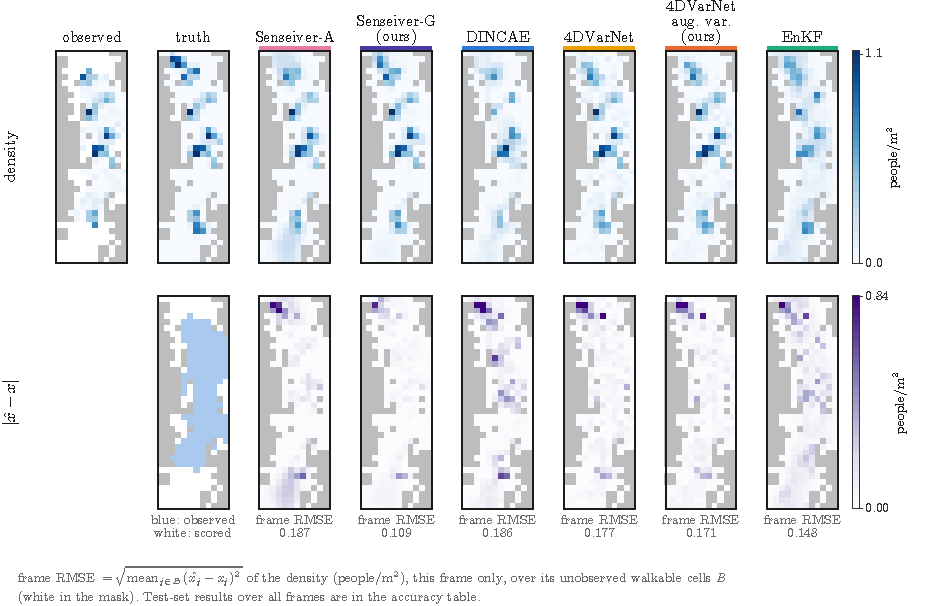
\includegraphics[width=\textwidth]{figures/comparison.pdf}
	\caption{Reconstructions of one test frame (11 August 2013, a busy second).
	Top: the robots' observation (unobserved cells white), the ground truth and
	the density reconstructed by each method, on one colour scale. Bottom: the
	absolute error of each reconstruction, on one colour scale; the leftmost
	panel shows the observed (blue) and the scored, unobserved (white) walkable
	cells. The frame RMSE under each panel is the density RMSE of this frame on
	its unobserved walkable cells.}
	\label{fig:comparison}
\end{figure}

%% ------------------------------------------------------------------
\subsection{Where the error comes from}
\label{sec:res_breakdown}

The pooled RMSE of Section~\ref{sec:res_acc} averages over very different
situations. To see where the methods differ, the error is broken down in three
ways (Figure~\ref{fig:breakdown}) and by whether a cell is occupied
(Table~\ref{tab:occupancy}). The breakdowns use the blind cells, where the state
must be inferred rather than read from an observation. For these breakdowns all six methods are scored on
the same frames, those of the uncertainty protocol (Section~\ref{sec:eval}), so
that within every group the methods are compared on identical cells; on these
frames the pooled RMSE values (0.206, 0.182, 0.215, 0.213, 0.277 and 0.235, in
the order of Table~\ref{tab:accuracy}) differ from the blind-cell values of
Table~\ref{tab:accuracy} by less than 1\%.

\begin{figure}[htb]
	\centering
	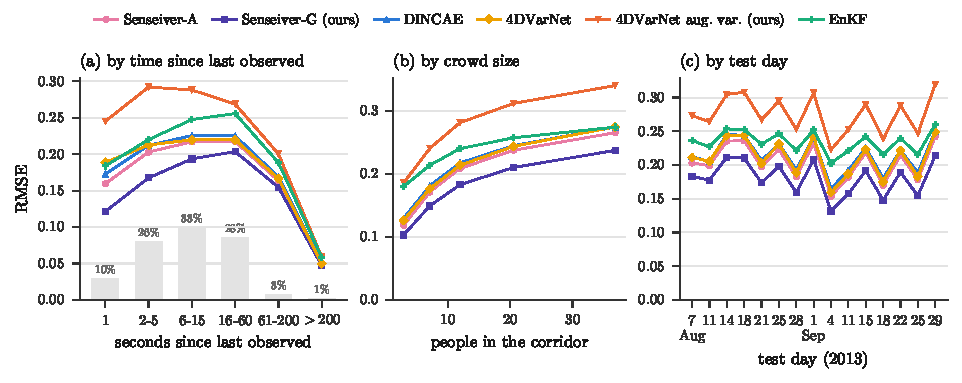
\includegraphics[width=\textwidth]{figures/breakdown.pdf}
	\caption{Reconstruction RMSE on the blind cells, pooled over the four
	channels, on the frames common to all six methods. (a) By the time since the
	blind cell was last observed; the grey bars and percentages give the share of
	the blind cells in each group. (b) By the number of people in the corridor at
	that second; the frames are grouped by quintiles of crowd size, placed at
	their mean number of people. (c) On each of the 15 test days.}
	\label{fig:breakdown}
\end{figure}

\paragraph{Time since the cell was last observed.}
Figure~\ref{fig:breakdown}a groups the blind cells by how long ago they were
last observed. For every method the error is higher for cells last observed
2--5\,s earlier than for those observed one second earlier, and for every method
except the augmented 4DVarNet it is higher again at 6--15\,s, which is consistent
with recent observations being informative; the groups contain different cells and crowd conditions, so the
figure does not isolate the effect of the elapsed time itself. The error decreases again for the few cells that have not
been observed for more than a minute (3\% of the blind cells), and is small
for the fewer than 1\% not observed for more than 200\,s. The advantage
of Senseiver\nobreakdash-G over Senseiver\nobreakdash-A is concentrated in the
recently observed cells: its RMSE is 24\% lower for cells observed one second
earlier, 17\% lower for 2--5\,s, 11\% lower for 6--15\,s, and about 6\% lower for
cells last observed 16--200\,s earlier, which no longer have a token of
their own in its 16-second window. For the fewer than 1\% of cells
unobserved for longer, the two methods have nearly the same RMSE (2\% apart). This
is consistent with Senseiver\nobreakdash-G benefiting from recent observations. The EnKF behaves differently from the
learned methods. For cells observed one second earlier it is slightly more
accurate than 4DVarNet (0.184 against 0.189); but whereas the error of Senseiver\nobreakdash-A, DINCAE
and 4DVarNet levels off after a few seconds (at about 0.22--0.23), that of the EnKF
keeps growing, to 0.248 at 6--15\,s and 0.256 at 16--60\,s.

\paragraph{Crowd size.}
The error of every method grows with the number of people in the corridor
(Figure~\ref{fig:breakdown}b), and Senseiver\nobreakdash-G is the most accurate method in
all five groups, followed by Senseiver\nobreakdash-A. For the learned methods other than the
augmented 4DVarNet, the RMSE is 2.1 to 2.3 times as large in the most crowded fifth
of the frames (37 people on average) as in the emptiest (3 people): the RMSE of
Senseiver\nobreakdash-G rises from 0.103 to 0.237. The EnKF is much less sensitive, rising
only from 0.180 to 0.274. In the least crowded group only the augmented
4DVarNet has a higher error than the EnKF, whereas in the most crowded group the EnKF is as
accurate as DINCAE and 4DVarNet (0.274 for all three).

\paragraph{Test days.}
Figure~\ref{fig:breakdown}c shows the methods on each of the 15 test days.
Senseiver\nobreakdash-G is the most accurate method on every day, by between 9.8\% and
14.2\% relative to Senseiver\nobreakdash-A, which is second on every day. 4DVarNet is ahead
of DINCAE on 12 of the 15 days, by small margins (Section~\ref{sec:res_acc}),
and the EnKF and the augmented 4DVarNet are fifth and sixth on every day. The
level of the error varies from day to day, for Senseiver\nobreakdash-G between 0.132 and
0.214, but it varies in the same way for all methods.

\paragraph{Empty and occupied cells.}
Of the scored blind cells, 83\% are empty in the ground truth.
Table~\ref{tab:occupancy} gives the density RMSE separately for empty and
occupied cells. On the occupied cells, the EnKF is the most accurate method
(0.257, against 0.263 for Senseiver\nobreakdash-G and at least 0.303 for the others); its
weakness is in the empty cells, where its error (0.084) is more than twice that
of Senseiver\nobreakdash-G (0.038). The EnKF therefore has a low density RMSE on occupied
cells but a larger error on empty cells, consistent with the positive density
reconstructed in some empty cells in
Figure~\ref{fig:comparison}. 4DVarNet has a similarly large error on the empty
cells (0.086), without the EnKF's accuracy on the occupied ones, and the
augmented 4DVarNet has the largest error on both (0.101 and 0.324). For
Senseiver\nobreakdash-A, Senseiver\nobreakdash-G and DINCAE, 87\% to 91\% of the squared density error
comes from the occupied sixth of the cells.

\begin{table}[htb]
	\centering
	\caption{Density RMSE on blind cells that are empty and that are occupied in
	the ground truth (people per m$^2$), on the frames common to all methods, and
	the share of the total squared density error that comes from the occupied
	cells. Occupied cells are 17\% of the scored cells.}
	\label{tab:occupancy}
	\small
	\begin{tabular}{lccc}
		\hline
		Method & Empty cells & Occupied cells & Share from occupied \\
		\hline
		Senseiver\nobreakdash-A                 & 0.052 & 0.303 & 87\% \\
		Senseiver\nobreakdash-G (ours)          & \textbf{0.038} & 0.263 & 91\% \\
		DINCAE                      & 0.054 & 0.310 & 87\% \\
		4DVarNet                    & 0.086 & 0.319 & 74\% \\
		4DVarNet aug.\ var.\ (ours) & 0.101 & 0.324 & 68\% \\
		EnKF                        & 0.084 & \textbf{0.257} & 65\% \\
		\hline
	\end{tabular}
\end{table}

\paragraph{The augmented 4DVarNet.}
The augmented 4DVarNet has the largest error in every crowd-size group, on
every test day, and in every group by the time since the last observation,
except the cells never observed that day (fewer than 0.01\% of the blind cells), where the EnKF's error is larger.
Its excess over the plain 4DVarNet peaks at 2--5\,s (0.080, against 0.056 at one
second) and shrinks for cells unobserved for longer (0.068 at 6--15\,s, 0.049 at
16--60\,s and 0.010 beyond 200\,s).

%% ------------------------------------------------------------------
\subsection{Uncertainty quality}
\label{sec:res_unc}

Table~\ref{tab:uncertainty} and Figure~\ref{fig:uncertainty} give the CRPS and
the spread/RMSE ratio of the three probabilistic methods, pooled with their 95\%
bootstrap intervals over test days, and per channel, on all walkable cells and
on the blind cells. The paragraphs below refer to the blind cells, except where
all walkable cells are stated.

\begin{table}[htb]
	\centering
	\caption{Uncertainty quality of the three probabilistic methods on all
	walkable cells, observed and blind (top), and on the blind cells (bottom),
	of the common frames of the 15 test days. Per-channel CRPS uses
the channel's physical unit; pooled CRPS has no single physical unit.
Lower CRPS is better. RMS spread / point-estimate RMSE measures overall scale,
with 1 as the reference size. Pooled values with 95\% bootstrap intervals over test days in
	brackets.}
	\label{tab:uncertainty}
	\small
	\setlength{\tabcolsep}{3pt}
	\begin{tabular}{llccc}
		\hline
		& & DINCAE & 4DVarNet aug.\ var.\ (ours) & EnKF \\
		\hline
		\multicolumn{5}{l}{\emph{All walkable cells}} \\
		CRPS        & All    & \textbf{0.055} {\small [0.049, 0.060]} & 0.084 {\small [0.080, 0.088]} & 0.072 {\small [0.068, 0.076]} \\
		            & $\rho$ & 0.037 & 0.046 & \textbf{0.035} \\
		            & $v_x$  & \textbf{0.113} & 0.209 & 0.150 \\
		            & $v_y$  & \textbf{0.049} & 0.063 & 0.064 \\
		            & $\nu$  & 0.019 & \textbf{0.018} & 0.040 \\
		\hline
		Spread/RMSE & All    & 0.57 {\small [0.39, 0.81]} & 1.17 {\small [1.13, 1.21]} & 1.26 {\small [1.22, 1.31]} \\
		            & $\rho$ & 0.86 & 1.24 & 0.94 \\
		            & $v_x$  & 0.82 & 1.04 & 1.29 \\
		            & $v_y$  & 0.88 & 1.08 & 1.50 \\
		            & $\nu$  & 0.15 & 2.78 & 0.93 \\
		\hline
		\multicolumn{5}{l}{\emph{Blind cells}} \\
		CRPS        & All    & \textbf{0.069} {\small [0.062, 0.075]} & 0.096 {\small [0.089, 0.103]} & 0.086 {\small [0.082, 0.090]} \\
		            & $\rho$ & 0.046 & 0.056 & \textbf{0.039} \\
		            & $v_x$  & \textbf{0.141} & 0.228 & 0.169 \\
		            & $v_y$  & \textbf{0.063} & 0.073 & 0.077 \\
		            & $\nu$  & \textbf{0.024} & 0.026 & 0.058 \\
		\hline
		Spread/RMSE & All    & 0.83 {\small [0.80, 0.87]} & 1.08 {\small [1.04, 1.12]} & 1.27 {\small [1.23, 1.32]} \\
		            & $\rho$ & 0.93 & 1.02 & 0.97 \\
		            & $v_x$  & 0.82 & 0.91 & 1.30 \\
		            & $v_y$  & 0.87 & 0.94 & 1.53 \\
		            & $\nu$  & 0.72 & 2.54 & 0.96 \\
		\hline
	\end{tabular}
\end{table}

\begin{figure}[htb]
	\centering
	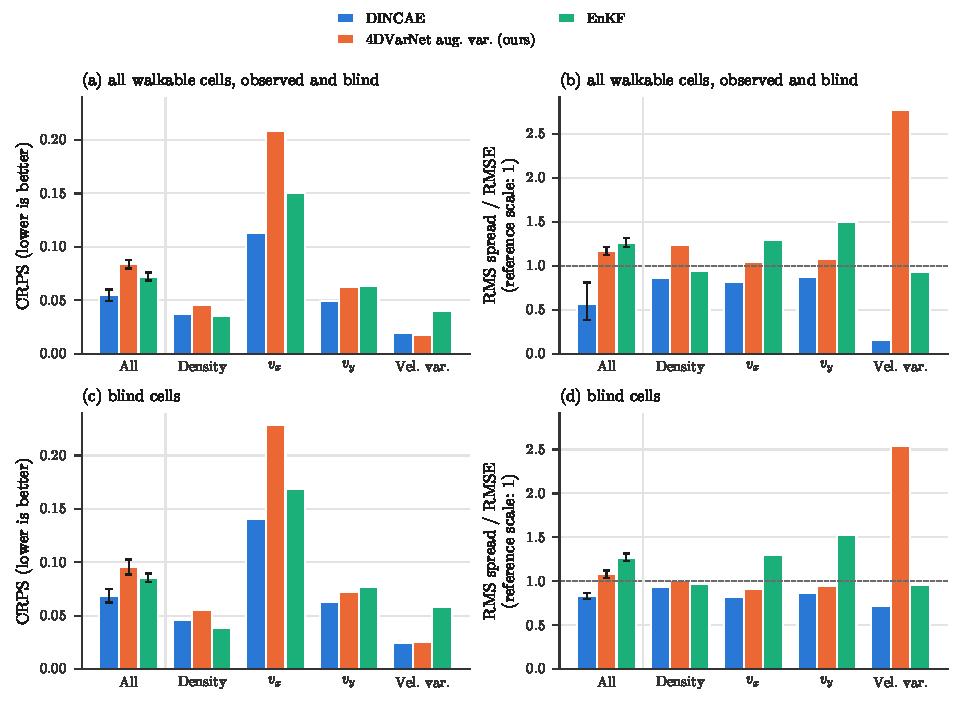
\includegraphics[width=\textwidth]{figures/uncertainty.pdf}
	\caption{Uncertainty quality of the three probabilistic methods, pooled over
	the four channels (left group) and per channel, on all walkable cells,
	observed and blind (a, b), and on the blind cells (c, d). (a, c) CRPS;
	per-channel CRPS has the channel's physical unit, pooled CRPS has no single
	physical unit (lower is better). (b, d) RMS predictive spread /
	point-estimate RMSE, with the dashed line at 1 marking equal overall scale.
	Error bars on the pooled values: 95\% bootstrap intervals over the 15 test
	days.}
	\label{fig:uncertainty}
\end{figure}

\paragraph{CRPS.}
DINCAE has the lowest CRPS, pooled (0.069) and on three of the four channels;
its bootstrap interval does not overlap those of the EnKF (0.086) and the
augmented 4DVarNet (0.096), and it has the lowest CRPS on each of the 15 test
days, so its lead persists across this test split. On the density alone the
EnKF is better (0.039 against DINCAE's 0.046). The augmented 4DVarNet has the
highest pooled CRPS; its interval overlaps that of the EnKF, but the EnKF has
the lower CRPS on 14 of the 15 test days. Per channel, the augmented 4DVarNet
is behind the EnKF on the density and $v_x$ and ahead of it on $v_y$ and the
velocity variance. DINCAE's point estimate is also the most accurate of the
three on the blind cells (Table~\ref{tab:accuracy}), so its lower CRPS
reflects the predictive distribution as a whole and not necessarily a better
uncertainty alone.

\paragraph{Size of the predicted uncertainty.}
DINCAE's RMS predictive spread is 0.83 times the pooled point-estimate
RMSE: 0.93 on density, 0.82 and 0.87 on the two velocity components, and 0.72
on the velocity variance. These are overall scale ratios rather than
statements about every cell.

The EnKF has a pooled spread/RMSE ratio above one (1.27). Its ratios are 1.30 for $v_x$
and 1.53 for $v_y$, while density and the velocity variance are close to the
reference scale (0.97 and 0.96).

The augmented 4DVarNet has the pooled ratio closest to one (1.08), but this
hides a mismatch between the channels: its spread is close to the reference
scale on density (1.02), slightly small on the two velocity components (0.91
and 0.94), and 2.54 times its error on the velocity variance.

\paragraph{All walkable cells.}
On all walkable cells, where the observed cells are scored too, the ranking by
CRPS is the same as on the blind cells: DINCAE (0.055) is ahead of the EnKF
(0.072) and the augmented 4DVarNet (0.084), in this order on each of the 15
test days. Per channel, the EnKF has the lowest CRPS on the density and the
augmented 4DVarNet on the velocity variance. The spread/RMSE ratios of the EnKF
and the augmented 4DVarNet (1.26 and 1.17) are close to their blind-cell values
(1.27 and 1.08). DINCAE's ratio, 0.57 with a wide interval from 0.39 to 0.81,
is not: in a few observed cells its unclipped velocity-variance mean leaves the
fixed range $[0, 2]$ by orders of magnitude. Over the 15 test days, 6\,781 of its 93
million scored velocity-variance values on observed cells (0.007\%) lie more
than one range width outside $[0, 2]$, and in 72\% of these cells the ground
truth itself exceeds 2: they are cells with extreme velocity-variance records,
which DINCAE receives as observations. The largest prediction, on 18 September,
is 3\,786 against a true value of 29.9. Because the uncertainty is scored without
clipping (Section~\ref{sec:eval}), these values dominate DINCAE's RMSE on all
walkable cells (0.258, against 0.176 for its clipped point estimate in
Table~\ref{tab:accuracy}) and with it the spread/RMSE ratio, whereas the CRPS
grows only linearly with the error. On the blind
cells, only 109 such values occur.

\paragraph{Coverage of the prediction intervals.}
Table~\ref{tab:coverage} checks how often the stated intervals contain the
truth. On the blind cells, the intervals of DINCAE and the augmented 4DVarNet
contain the truth more often than the nominal 50\% on both the density and the
velocity (0.83 and 0.73 on the density, 0.76 and 0.67 on the velocity), and at about or
above the nominal 90\% (0.96 and 0.93 on the density, 0.92 and 0.90 on the velocity). The
intervals of the EnKF contain the truth less often than stated on the density
at both levels (0.40 and 0.77), and on the velocity at the 90\% level (0.82),
whereas its 50\% interval on the velocity is at the nominal value (0.51); its
RMS spread on the blind cells is 0.97 times its error on the density and larger
than its error on the velocity. On the velocity variance, the same pattern
holds: on the blind cells, DINCAE reaches 0.81 and 0.98, the augmented 4DVarNet
0.80 and 0.96, and the EnKF 0.30 and 0.79, the lowest 50\% coverage in
the table. On all walkable cells, the EnKF again has the lowest coverage on
every channel, and DINCAE is above the augmented 4DVarNet except at the 50\%
level on the velocity variance (0.74 against 0.80).
These fractions pool empty and occupied cells, and 83\% of the scored blind
cells are empty (Section~\ref{sec:res_breakdown}); the coverage was not computed
separately for the two.

\begin{table}[htb]
	\centering
	\caption{Coverage of the central 50\% and 90\% prediction intervals: the
	fraction of true values inside the interval, on the common frames of the 15
	test days, for the density, the two velocity components together and the
	velocity variance. The nominal values are 0.50 and 0.90.}
	\label{tab:coverage}
	\small
	\setlength{\tabcolsep}{4pt}
	\resizebox{\textwidth}{!}{%
	\begin{tabular}{lcccccc|cccccc}
		\hline
		& \multicolumn{6}{c|}{All walkable cells} & \multicolumn{6}{c}{Blind cells} \\
		\cline{2-13}
		& \multicolumn{2}{c}{$\rho$} & \multicolumn{2}{c}{$v_x, v_y$} & \multicolumn{2}{c|}{$\nu$} & \multicolumn{2}{c}{$\rho$} & \multicolumn{2}{c}{$v_x, v_y$} & \multicolumn{2}{c}{$\nu$} \\
		Method & 50\% & 90\% & 50\% & 90\% & 50\% & 90\% & 50\% & 90\% & 50\% & 90\% & 50\% & 90\% \\
		\hline
		DINCAE & 0.73 & 0.95 & 0.69 & 0.93 & 0.74 & 0.97 & 0.83 & 0.96 & 0.76 & 0.92 & 0.81 & 0.98 \\
		4DVarNet aug.\ var.\ (ours) & 0.65 & 0.92 & 0.61 & 0.91 & 0.80 & 0.96 & 0.73 & 0.93 & 0.67 & 0.90 & 0.80 & 0.96 \\
		EnKF & 0.38 & 0.76 & 0.56 & 0.86 & 0.42 & 0.82 & 0.40 & 0.77 & 0.51 & 0.82 & 0.30 & 0.79 \\
		\hline
	\end{tabular}}
\end{table}

\paragraph{Spatial structure.}
Figure~\ref{fig:uncertainty_maps} compares the absolute error with the predicted
$\hat{\sigma}$ in one test frame, on a shared colour scale. DINCAE's $\hat{\sigma}$ is smooth and high at the two ends of
the corridor, which the robots visit least often (Figure~\ref{fig:observation}b),
and around the occupied cells.
The EnKF's spread is high over most of the corridor, including cells where its
error is small; on the density, its spread nevertheless has about the size of
its error on average (0.97). The augmented 4DVarNet's $\hat{\sigma}$ is highest
in and around the occupied cells and low in the empty parts of the corridor; at
the group at the upper end, where its error is largest, its $\hat{\sigma}$ is
clearly smaller than the error.

\begin{figure}[htb]
	\centering
	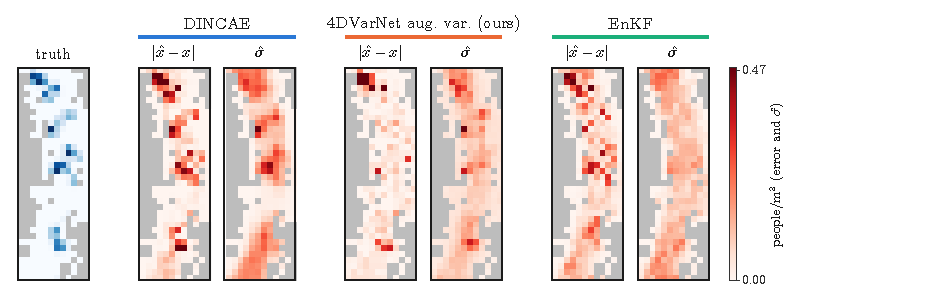
\includegraphics[width=\textwidth]{figures/uncertainty_maps.pdf}
	\caption{Absolute density error $|\hat{x} - x|$ and predicted $\hat{\sigma}$
	of the three probabilistic methods in the test frame of
	Figure~\ref{fig:comparison}, with the ground truth for reference. Error and
	$\hat{\sigma}$ share one colour scale for a qualitative spatial comparison.
Calibration is assessed over the scored cells and frames, rather than inferred
from this single realisation.}
	\label{fig:uncertainty_maps}
\end{figure}

%% ------------------------------------------------------------------
\subsection{Computational cost}
\label{sec:res_cost}

Figure~\ref{fig:latency} gives the median compute time per reconstructed frame
on a GPU. The
methods span more than two orders of magnitude: DINCAE needs 0.030\,ms per
frame, Senseiver\nobreakdash-A 0.145\,ms, 4DVarNet 0.31\,ms, the augmented 4DVarNet
0.39\,ms, Senseiver\nobreakdash-G 0.82\,ms and the EnKF 7.3\,ms. The EnKF, which at every second
propagates 100 ensemble members through its forecast model and computes an
analysis, is the slowest. Senseiver\nobreakdash-G is 5.7 times slower than
Senseiver\nobreakdash-A, because its encoder attends from 432 cell tokens instead of 64
latents and reads the tokens of up to 16\,s instead of 1\,s. Even the
slowest method is more than a hundred times faster than the rate at which the
observations arrive, one frame per second, so on this GPU compute is not the binding
constraint for any of them. Compute time is not the same as availability: these
are throughputs per output frame, measured with the inputs prepared beforehand
and, for Senseiver and DINCAE, in batches, whereas the EnKF must advance one
second at a time. Three of the methods also have to wait for observations that
are later than the frame they reconstruct -- one second for DINCAE, and up to
199\,s, 99.5\,s on average, for a frame inside a 200-second window of either
4DVarNet model.
Only the three causal methods, Senseiver\nobreakdash-A, Senseiver\nobreakdash-G and the EnKF, can deliver the current frame as soon as its observation arrives.

\begin{figure}[htb]
	\centering
	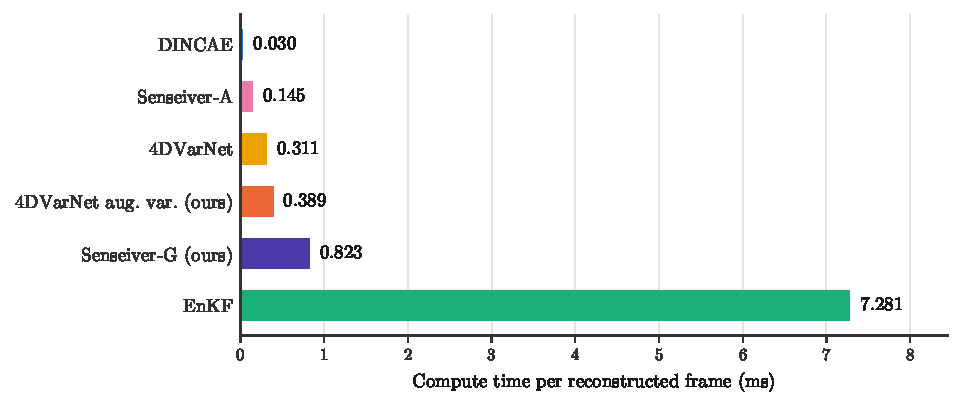
\includegraphics[width=\textwidth]{figures/latency.pdf}
	\caption{Median compute time per reconstructed frame over three timing
	runs on one NVIDIA Tesla V100-SXM2-16GB. Inputs are prepared from the
	same held-out 600-frame block with each method's required context.
	Bar lengths use a linear scale starting at zero; labels give milliseconds
	to three decimal places. The two 4DVarNet models reconstruct 200-frame
	windows, and their time is divided by 200; the EnKF propagates 100 members.
	These values measure per-frame compute cost, rather than the waiting
	time for an individual result.}
	\label{fig:latency}
\end{figure}

%% ------------------------------------------------------------------
\subsection{Discussion}
\label{sec:discussion}

\paragraph{RQ1: reconstruction accuracy.}
Among the six methods, the proposed Senseiver\nobreakdash-G reconstructs the state over
the walkable area most accurately, on every channel, with a pooled RMSE 12.7\%
below Senseiver\nobreakdash-A and 31.0\% below 4DVarNet on all walkable cells, and 11.7\%
and 14.5\% below them on the blind cells. On the blind cells, this holds on
each of the 15 test days and for every size of the crowd
(Section~\ref{sec:res_breakdown}). It is also obtained under the stricter
condition: DINCAE and the two 4DVarNet models use observations after the reconstructed frame
and could not deliver it online without delay, whereas Senseiver\nobreakdash-G uses only
current and past observations. The breakdown by the time since a blind cell was last observed
is consistent with the benefit of a short causal window: two thirds of the blind
cells have been observed within the last 15\,s, and it is on these cells
that Senseiver\nobreakdash-G gains the most, by up to 24\% for cells observed one second
earlier. The comparison does not separate the two changes of Senseiver\nobreakdash-G, the
grid-aligned latent array and the window: in the design selection, the comparison of
the latent arrays also changes the number
of latent vectors and the read-out, and the test comparison evaluates the
complete configuration. The EnKF is more accurate than
every method except Senseiver\nobreakdash-G on the density of the blind cells, and it has
the lowest density RMSE on the occupied cells, while its error on empty cells
is larger. Its RMSE is higher than Senseiver\nobreakdash-G's on every channel.
The second proposed model, the augmented 4DVarNet, is less accurate than the
plain 4DVarNet it extends (blind-cell RMSE 0.276 against 0.212), mostly on
$v_x$, and it is the least accurate of the six methods. The two runs share the
solver and the training seed and differ in the variance parts and in the
Gaussian likelihood they are trained with; in the reported runs, adding the
variance therefore came with a less accurate mean.

\paragraph{RQ2: uncertainty quality.}
Of the three methods that predict an uncertainty, DINCAE gives the
best-scoring probabilistic prediction: it has the lowest CRPS on every test day
and on three of the four channels. The CRPS scores the predictive distribution
as a whole, so this lead is not a statement about the variance alone: DINCAE's
point estimate is also the most accurate of the three on the blind cells (RMSE
0.214, against 0.235 for the EnKF and 0.276 for the augmented 4DVarNet), and
part of its advantage is that accuracy. Separating the two would require
scoring the same point estimate with and without the learned variance, which
was not done here. The EnKF follows (pooled CRPS 0.086, the lowest on the
density) and is ahead of the augmented 4DVarNet (0.096) on 14 of the 15 test
days. On all walkable cells the CRPS ranking is the same, while DINCAE's
spread/RMSE ratio there is distorted by a few extreme velocity-variance
predictions on observed cells (Section~\ref{sec:res_unc}). On the blind cells, in overall size, DINCAE's spread is smaller than its error (0.83) and the
EnKF's larger (1.27); the augmented 4DVarNet's pooled ratio is the closest to
one (1.08), but it combines a spread close to the error on the density and the
two velocity components with one 2.5 times the error on the velocity variance.
On the blind cells, the intervals of DINCAE and the augmented 4DVarNet contain
the truth at least as often as stated, and those of the EnKF
less often, except its 50\% interval on the velocity
(Table~\ref{tab:coverage}).
DINCAE provides both the lowest RMSE and the lowest pooled CRPS of the three
probabilistic methods, at about 1/250 of the EnKF's
compute time per reconstructed frame.

\paragraph{RQ3: computational cost.}
The six methods differ by a factor of about 250 in per-frame compute cost, from
0.030\,ms per frame for DINCAE to 7.3\,ms for the EnKF, with Senseiver\nobreakdash-A
(0.145\,ms), the two 4DVarNet models (0.31 and 0.39\,ms) and Senseiver\nobreakdash-G
(0.82\,ms) in between. The uncertainty output of the augmented 4DVarNet costs
25\% more compute time than the plain 4DVarNet (0.39 against 0.31\,ms), and
the augmented 4DVarNet needs about a nineteenth of the EnKF's time per frame.
The measured compute times of all six methods are below the
one-second interval between observations. DINCAE and both 4DVarNet models
nevertheless require future observations for a reconstructed frame, so they
cannot produce that frame without delay. The grid latent and the
temporal window make Senseiver\nobreakdash-G 5.7 times slower than Senseiver\nobreakdash-A. The most accurate method,
Senseiver\nobreakdash-G, and the method with the lowest pooled CRPS, DINCAE, are different,
and neither has the largest measured compute cost.

\paragraph{The trade-off of the augmented 4DVarNet.}
The augmented 4DVarNet adds an uncertainty to 4DVarNet within one invocation
of its trained solver, without an ensemble or repeated evaluations, for 25\%
more computation per frame (0.39 against 0.31\,ms). In the reported run, this
came with a less accurate mean: its blind-cell RMSE is 0.276 against 0.212 for
the plain 4DVarNet, mostly on $v_x$, and it is the least accurate of the six
methods. Of the three probabilistic methods, its predicted spread has the
pooled size closest to its error (spread/RMSE 1.08), but its CRPS is the
highest (0.096). This trade-off, an uncertainty from a single model at a cost
in accuracy, is part of the contribution of this thesis; whether the loss of
accuracy holds across training seeds was not measured.

\paragraph{Interpretation of the uncertainties.}
DINCAE and the augmented 4DVarNet estimate conditional predictive distributions
from a single trained model. Their variance outputs describe uncertainty in
the state given the supplied observations, as learned from training data;
parameter uncertainty is not explicitly estimated
\cite{kendall2017uncertainties}. Both use Gaussian distributions.

The EnKF's spread arises from propagation of the state ensemble, structured process
noise, and observation updates. Its members carry a joint sample covariance
across cells and channels, of rank at most $N_e-1$. The learned models output
marginal distribution parameters without a joint error covariance. This
evaluation scores per-cell marginals and does not assess the EnKF's joint
structure.

\paragraph{Limitations.}
The results hold for one setting: one corridor of one shopping centre, observed
by three robots with a sensing radius of seven cells that move independently of
the crowd. The ranking of the methods may change with the number of robots, the
sensing range, or robots that react to the crowd. The observations are
simulated, as the ground truth on the observed cells plus Gaussian noise of a
fixed, assumed size; real on-board sensing would add occlusion by pedestrians,
detection errors and errors in the robots' own localisation, and the ground
truth is itself the output of a tracking system. The methods also use different
temporal information: DINCAE and both 4DVarNet models use observations after
the reconstructed frame, so their accuracy is not directly comparable with
that of the causal methods for online use. Finally, each learned method is
represented by one final training run, and each test day by one realisation of
the robot routes, so the variability due to random initialisation and to the
routes is not measured. This matters most for Senseiver\nobreakdash-A, DINCAE and 4DVarNet,
whose pooled RMSEs on the blind cells are close (0.206, 0.214 and 0.212).

\clearpage

\section{Conclusions}
\label{sec:summary}

This thesis evaluated six methods for reconstructing a four-channel
macroscopic crowd field from partial, noisy observations of three simulated
mobile robots in the ATC corridor. It proposed Senseiver\nobreakdash-G, with a grid-aligned
latent representation and a causal temporal window, and an augmented 4DVarNet
that refines the state and its log-variance within one trained solver invocation.
The four existing methods could all be adapted to the crowd domain
(Section~\ref{sec:models}).

For reconstruction accuracy (RQ1), Senseiver\nobreakdash-G has the lowest RMSE on every
channel, on all walkable cells and on the blind cells, in the reported 15-day
test comparison. Its pooled RMSE on all walkable cells is 0.125, 12.7\% below
Senseiver\nobreakdash-A's and 31.0\% below 4DVarNet's 0.181; on the blind cells it is
0.182, 11.7\% and 14.5\% below theirs, using only current and past
observations. The augmented 4DVarNet is less accurate than the plain 4DVarNet
(0.276 against 0.212 on the blind cells) and the least accurate of the six
methods.

For predictive-distribution quality (RQ2), DINCAE has the lowest pooled CRPS
on the blind cells (0.069, against 0.086 for the EnKF and 0.096 for the
augmented 4DVarNet), helped by its more accurate point estimate, and the lowest
CRPS on all 15 test days, also on all walkable cells (0.055). On the blind cells, its RMS spread is 0.83 times its point-estimate RMSE, the EnKF's 1.27
times and the augmented 4DVarNet's 1.08 times; the last combines a spread close
to its error on the density and the velocities with one 2.5 times its error on
the velocity variance. On the blind cells, the 50\% and 90\% prediction intervals
of DINCAE and the augmented 4DVarNet contain the truth at least as often as
stated, and those of the EnKF contain it less often, except its 50\% interval on
the velocity.

For computational cost (RQ3), the measured time per reconstructed frame ranges from
0.030\,ms for DINCAE to 7.3\,ms for the EnKF. These are average per-frame
compute costs with prepared inputs. The augmented 4DVarNet needs 0.39\,ms, 25\%
more than the plain 4DVarNet and about a nineteenth of the EnKF's time.
DINCAE and both 4DVarNet models also need
future observations, whereas Senseiver\nobreakdash-G uses the available observations
causally.

\paragraph{Future work.}
The results suggest several directions.
\begin{itemize}
	\item \emph{A more accurate augmented 4DVarNet.} In the reported run, adding
	the variance came with a less accurate mean, mostly on $v_x$, and a spread
	of the velocity variance much larger than its error. Repeating the
	comparison with several seeds, and training the variance after the state
	or with less weight, would show whether this loss of accuracy is inherent
	to the joint training.
	\item \emph{Calibrating the predicted uncertainty.} On the blind cells,
	DINCAE's RMS spread is below its RMSE while its prediction intervals contain
	the truth more often than stated, and the EnKF's RMS spread is above its RMSE
	while its intervals mostly contain the truth less often; the augmented
	4DVarNet's spread is much larger than its error on the velocity variance. A
	per-channel rescaling of $\hat{\sigma}$, fitted on validation days, would
	therefore have to be checked against both measures.
	\item \emph{An uncertainty-aware causal model.} Senseiver\nobreakdash-G is the most
	accurate method but predicts no uncertainty; giving it a variance output
	trained with a likelihood, as in DINCAE, could provide a causal probabilistic
	reconstruction. Its effect on accuracy would need evaluation. Conversely, 4DVarNet could be made causal with
	windows that end at the reconstructed frame.
	\item \emph{Broader evaluation.} The ranking should be tested under different
	numbers of robots and sensing ranges, in other environments, and with
	several training runs per method, to separate the effect of the method from
	that of the random initialisation.
	\item \emph{Use in planning.} The purpose of an uncertainty estimate is to
	inform decisions. Using the predicted $\hat{\sigma}$ to direct the robots
	towards the cells where the reconstruction is least certain would close the
	loop between estimation and sensing, and would allow the uncertainty to be
	evaluated by the value of the decisions it supports.
\end{itemize}

\clearpage

%\DeclareFieldFormat{urldate}{%
%	(Accessed on %
%	\mkbibmonth{\thefield{urlmonth}}\addspace%
%	\thefield{urlday}\addcomma \addspace      %
%	\thefield{urlyear}\isdot)}

\printbibliography[heading=bibintoc]

\end{document}
